% !TeX spellcheck = en-UK
% Qui tutto ciò che c’ è da saper su LaTeX: http://www.lorenzopantieri.net/LaTeX_files/ArteLaTeX.pdf
% Per scrivere la bibliografia puoi vedere il seguente link: https://www.guitex.org/home/images/doc/GuideGuIT/bibliografia.pdf
% Per usare in locale questo progetto latex è necessario eseguire le seguenti installazioni:
% sudo apt install texlive texstudio texlive-publishers texlive-latex-extra texlive-fonts-extra texlive-science texlive-bibtex-extra texlive-lang-english

% Tipo di documento
\documentclass[oneside]{book}

% Pacchetti
\usepackage[letterpaper,top=2cm,bottom=2cm,left=3cm,right=3cm,marginparwidth=1.75cm]{geometry}
\usepackage[english]{babel}
\usepackage[utf8]{inputenc}
\usepackage{imakeidx}
\usepackage{appendix}
\usepackage{enumitem}
\usepackage{marginnote}
\usepackage{tocloft}
\usepackage{float}
%pacchetti matematici
\usepackage{amssymb}
\usepackage{mathtools}
\usepackage{amsmath}
\usepackage{amsthm}
\usepackage{siunitx}
% !ATTENZIONE: c'è un bug in thmtools, per approfondire vedere: https://tex.stackexchange.com/questions/305174/proof-environment-produces-proof-proof-only-when-thmbox-is-used
\usepackage{letltxmacro}
\LetLtxMacro\amsproof\proof
\LetLtxMacro\amsendproof\endproof
\usepackage{thmtools}
\AtBeginDocument{%
	\LetLtxMacro\proof\amsproof
	\LetLtxMacro\endproof\amsendproof
}
\usepackage{dsfont}
% pacchetti per le immagini
\usepackage{graphicx}
\usepackage{subcaption}
\usepackage{color}
\usepackage[dvipsnames, table]{xcolor}
% pacchetti per la scrittura di codice
\usepackage{listings}
\usepackage{algorithm}
\usepackage{algpseudocode}
\usepackage{algorithmicx}
\usepackage{marvosym}
% pacchetti per la gestione di citazioni e bibliografia
\usepackage[sort]{natbib}
% citazioni migliori
\usepackage[colorlinks=true]{hyperref}
\usepackage{cleveref}

% Settings
\bibliographystyle{plainnat} %ordine della bibliogragia
\setcitestyle{numbers}
\setcitestyle{square}
\definecolor{Teal}{rgb}{0.0, 0.5, 0.5}
\hypersetup{
    colorlinks=true,
    linkcolor=MidnightBlue,  % Un blu scuro, meno appariscente ma ben visibile
    citecolor=ForestGreen,   % Verde più scuro e tenue rispetto al verde brillante
    filecolor=RoyalPurple,   % Un viola meno intenso, che non è troppo chiaro
    urlcolor=Teal,           % Un colore verde-blu scuro, meno brillante del ciano
    pdftitle={Esempio di Documento},
    pdfauthor={Nome Autore},
    pdfkeywords={Latex, hyperref, hyperlink}
}

% Definizioni
\lstdefinestyle{code}{
    backgroundcolor=\color{white},
    commentstyle=\bfseries\itshape\color{gray},
    basicstyle=\ttfamily\scriptsize,
    keywordstyle=\color{blue},
    numberstyle=\tiny\color{gray},
    numbersep=5pt,
    stringstyle=\color{orange},
    showspaces=false,
    showstringspaces=false,
    showtabs=true,
    numbers=left,
    prebreak=\raisebox{0ex}[0ex][0ex]{\ensuremath{\hookleftarrow}},
    captionpos=t,
    frame=bottomline,
    breakatwhitespace=true,
    breaklines=true,
    keepspaces=true,
    tabsize=2,
    escapeinside={\%*}{*)}
}

\declaretheorem[
    name=Remark,
    numbered=no,
    style=remark
]{remark}
\declaretheorem[
    name=Exempli Gratia,
    numbered=no, shaded,
    style=remark
]{exempli_gratia}
\declaretheorem[
    name=Definition,
    numberwithin=section, shaded,
    style=definition
]{definition}
\declaretheorem[
    name=Notation,
    numbered=no, shaded,
    style=definition
]{notation}
\declaretheorem[
    name=Theorem,
    numberwithin=chapter, thmbox=M,
    style=plain
]{theorem}
\declaretheorem[
    name=Proposition,
    numberwithin=chapter,
    style=plain
]{proposition}
\declaretheorem[
    name=Lemma,
    numberwithin=section,
    style=plain
]{lemma}
\declaretheorem[
    name=Corollary,
    numbered=no,
    style=plain
]{corollary}

\algnewcommand{\Where}[2]{\State \textbf{where}\ #1\ \textbf{do} #2}

\definecolor{mint}{rgb}{0.88, 1.0, 0.88}
\definecolor{lavender}{rgb}{0.9, 0.9, 0.98}
\definecolor{honeydew}{rgb}{0.94, 1.0, 0.94}

\DeclareMathOperator{\sgn}{sgn}
\DeclareMathOperator{\lse}{lse}
\DeclareMathOperator{\softmax}{softmax}
\DeclareMathOperator{\const}{const}
\DeclareMathOperator{\argmin}{argmin}
\DeclareMathOperator{\argmax}{argmax}
\DeclareMathOperator{\diagonal}{diag}
\DeclareMathOperator{\accumulation}{acc}
\DeclareMathOperator{\closure}{cl}
\DeclareMathOperator{\internal}{int}
\DeclareMathOperator{\constant}{const}

\newcommand{\mathdef}{\coloneqq}
\newcommand{\upeq}[1]{\overset{#1}{=}}
\newcommand{\subapprox}[1]{\underset{#1}{\approx}}

% Sorgenti
\includeonly{
    glossary,
    bibliography,
    main/Introduction,
    main/DiscreteHopfield,
    main/ContinueHopfield,
    main/Applications,
    main/Conclusions,
}

\makeindex  % produce l'indice

\title{Continuous Hopfield Networks}
\author{
    Marcello Catacchini
    \and
    Stefano Magrini Alunno
    \and
    Dario Ferracci
}
\date{\today}

\begin{document}

\frontmatter
    \maketitle
    \tableofcontents

\mainmatter
	\setcounter{page}{1}
    \chapter{Introduction}
\label{ch:introduction}

% Introduzione del contesto storico del machine learning
Neural networks found their roots in the $1940$s, when Norbert Wiener introduced the concept of cybernetics with his book \textit{Cybernetics: Or Control and Communication in the Animal and the Machine}. The goal of cybernetics was to mimic natural systems to create mathematical models that could support the development of artificial intelligences. In particular, the attempt to replicate biological neural networks proved to be an attractive goal not only for mathematics, but also for many other disciplines. \footnote{For more about cybernetics, see \url{https://en.wikipedia.org/wiki/Cybernetics:_Or_Control_and_Communication_in_the_Animal_and_the_Machine}}

\noindent In the $1950$s, Frank Rosenblatt defined the perceptron in his article \textit{The perceptron: A probabilistic model for information storage and organization in the brain}, the first example of a neural network capable of autonomous learning to classify data. Despite its many limitations, the perceptron was an important starting point for understanding the direction of neural network research.

\noindent In the $1980$s, John Hopfield in his article \textit{Neural networks and physical systems with emergent collective computational abilities} proposed the first example of a neural network with an associative memory function. As time went on, researchers succeeded better and better in mimicking some of the basic functions of the human brain. Hopfield's networks were able to reconstruct or recall patterns without the use of indexical systems: the network stored information in a distributed manner and was able to retrieve it independently.

\noindent In the $1980$s, the backpropagation algorithm was also developed, marking a breakthrough for training feedforward networks and opening the door to deep learning \footnote{For more about backpropagation, see \textit{Applications of advances in nonlinear sensitivity analysis} of Paul J. Werbos}. In the $1990$s, convolutional networks (CNNs) and recurrent networks (RNNs), specific models that address practical application needs of neural networks, are introduced. Finally, thanks to technological advancement and the availability of more computational resources since 2010, it has become possible to effectively explore deep neural networks, revealing their extraordinary potential.

% Importanza storica delle reti di hopfield nel machine learning
\bigskip\noindent Hopfield networks introduced the possibility of storing patterns nonsequentially, making it possible to retrieve incomplete or noisy information. The network can recognize a pattern even if it is presented with a partial or distorted version, as human memory does when it recognizes a familiar face or object. This concept was novel compared to “addressed” memory systems, opening new avenues for implementing more flexible patterns.

\noindent Hopfield networks represented an example of distributed memory, in which every neuron in the network participates in the storage process. Unlike centralized memory systems, information in a Hopfield network is distributed among all synaptic connections, which makes it resistant to local errors and increases storage capacity.

\noindent Despite limitations in scalability, Hopfield networks have been successfully used to solve combinatorial optimization problems, such as the traveling salesman problem. The novel approach of Hopfield networks has inspired further developments in recurrent networks and associative memories, also influencing applications of modern recurrent neural networks.

\noindent Hopfield networks, while fundamental, had limitations such as low storage capacity and difficulty scaling to complex problems. However, they provided a strong impetus for subsequent research, leading to the development of more advanced architectures such as Boltzmann networks and deep neural networks, which built on their insight to solve increasingly complex problems.

% Sviluppo del machine learning
\bigskip\noindent In recent decades, the development of neural networks has increasingly turned toward feedforward models and deep neural networks. These models are based on a layered structure in which neurons, organized in different layers, process information sequentially. Unlike recurrent and associative networks, feedforward networks do not have internal loops, allowing information to be handled in a simple and linear manner, making them suitable for classification and regression tasks.

\noindent Deep networks make extensive use of logits, real numeric values that represent the activation of each neuron with respect to a certain input. These logits indicate how much a neuron “believes” the input to be similar to a specific class or feature, allowing the network to make decisions at different levels of abstraction.

\noindent This statistical approach, which relies on the activation of neurons through logits, is the basis of modern backpropagation and learning algorithms, making neural networks increasingly accurate and flexible in solving complex problems.

% Sviluppo delle reti di Hopfield continue
\bigskip\noindent The analysis of continuous Hopfield networks proves fundamental to understanding the evolution of modern neural architectures. Unlike their discrete counterparts, these networks can directly incorporate the concept of backpropagation, allowing continuous optimization of weights through gradient activation functions.

\noindent Continuous Hopfield networks introduce smoother dynamics in pattern representation and information retrieval, improving learning ability compared to discrete models. This aspect is highlighted in the article \textbf{“Hopfield Networks Are All You Need”}, where the authors explore how these networks can support more complex and adaptive learning functions.

\noindent In addition, continuous Hopfield networks lay the foundation for the adoption of advanced techniques, such as deep neural networks, which make use of more sophisticated learning algorithms. Therefore, the evolution from discrete to continuous Hopfield networks offers important insights for research and application in the field of machine learning.

% Cosa facciamo in questo articolo
\bigskip\noindent In this article, we will explore the applications of Hopfield networks in advanced contexts. We will begin by examining discrete Hopfield networks in detail, explaining their foundational mechanisms and functionality, as well as their connections to statistical mechanics. Additionally, we will focus on using Hopfield networks for data cleaning, demonstrating how effective results can be achieved with minimal parameterization, a concept that parallels techniques in convolutional neural networks (CNNs).

\noindent We will highlight how Hopfield networks can be employed for pattern management and reconstruction, allowing information retrieval even in the presence of noisy or incomplete data.

\noindent In addition, we will analyze continuous and stochastic Hopfield networks, studying their relationships with Variational Autoencoders (VAEs) and how these interactions can further expand their scope in contemporary machine learning.

\noindent Through these explorations, we intend to illustrate the potential of Hopfield networks not only as theoretical models, but as practical tools to address specific challenges in data preprocessing and performance improvement in learning models.

    \chapter{Discrete Hopfield Networks}
\label{ch:DHopfield}

In this chapter we are going to resume the notes of the course of Mathematical Models for Neural Networks of \citet{MMNN}. In particular, we are going to talk about the derivation of Hopfield neural networks and their properties. We are going to start from the derivation as a neural network with discrete states and finally we are going to use the perspective of statistical mechanics to analyze these neural networks.

\section{Derivation}

It's possible to make a mathematical model in order to analyze a natural neural network. Each neuron is a node of a graph and each synapse is an edge. A neural network is thus a graph.

\noindent Let two neurons, $A$ and $B$, be linked by a synapse. With respect to neuron $A$, we say that $A$ is a post-synaptic neuron and $B$ is a pre-synaptic neuron. A post-synaptic neuron receives information from all possible pre-synaptic neurons. This information consists of positive or negative ions, or even hormones that stimulate or alter the behavior of the neuron. In particular, these neurotransmitters either increase or decrease the potential of the neuron. If this potential exceeds a threshold, the neuron sends a message to the post-synaptic neurons and resets the potential. In \cref{fig:simple_diagram}, we show a simple diagram of the interaction between pre-synaptic and post-synaptic neurons.
\begin{figure}[htbp]
    \centering
    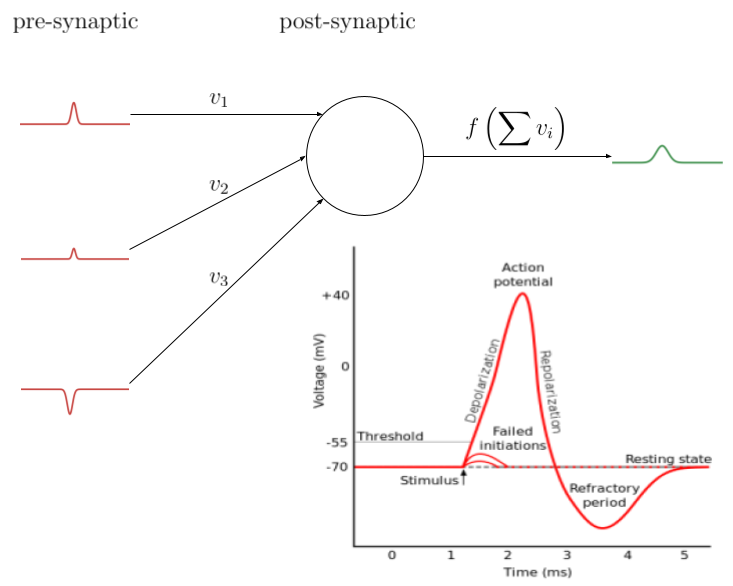
\includegraphics[width=0.8\linewidth]{Figures/simple_diagram.png}
    \caption{Pre-synaptic neurons send a signal to the post-synaptic neuron as a change in potential. The post-synaptic neuron accumulates all signals and generates a new signal if its potential exceeds a threshold.}
    \label{fig:simple_diagram}
\end{figure}
\begin{notation} In this article we denote with:
    \begin{itemize}
        \item[$U_i^t$] The potential of ${i}^\mathrm{th}$ neuron at time $t$.
        \item[$S_i^t$] The signal of ${i}^\mathrm{th}$ neuron at time $t$ from post-synaptic neurons.
        \item[$U_i^\star$] the threshold of ${i}^\mathrm{th}$ neuron.
        \item[$J$] The matrix of weights, where $J_{ij}$ is the weight over the synapse from $i$ to $j$.
        \item[$\theta$] The activation function ($0$ if the argument is not positive, $1$ otherwise).
    \end{itemize}
\end{notation}
\begin{definition}[interaction] We define the interaction rule with following formula, using the \textbf{McCulloch-Pitts} model:
    \begin{align}
        & U_i^t = \sum_j J_{ij}S_j^t \in \left[0, \sum_j J_{ij}\right]\\
        & S_i^{t+1} = \theta \left[U_i^t - U_i^\star\right] \in \{0,1\}
    \end{align}
    It's possible to get a different interpretation using only signals:
    \[
        S_i^{t+1} = \theta \left[\sum_j J_{ij}S_j^t - U_i^\star\right]
    \]
    then, we define \textbf{Ising} model, where the signal is $\xi_i^t = 2S_i^t-1\in\{-1,1\}$ and \\
    the threshold is $h_i = \sum_j J_{ij} - 2U_i^\star$:
    \begin{equation}
        \xi_i^{t+1} = \sgn \left[\sum_j J_{ij}\xi_j^{t} + h_i\right]
    \end{equation}
\end{definition}

\bigskip\noindent We define the interaction, but not the update of the entire neural network. In this article, we use both parallel and sequential dynamics, which are defined as follows:
\begin{definition}[updating] \label{def:discupdating} We use matrix notation as follows:\\
\textbf{Parallel dynamics}:
    \[
        \xi^{t+1} = \sgn\left[J\xi^t+h\right]
    \]
     All neurons are updated in parallel after one iteration.\\
\textbf{Sequential dynamics}:\\
Choose $i$ randomly:
     \[
        \xi_i^{t+1} = \sgn \left[\sum_j J_{ij}\xi_j^{t} + h_i\right]
    \]
    Only one neuron is updated at a time in sequential dynamics.

    \bigskip \noindent Where $\xi^t$ is the vector of all neurons' states (or Ising spins). Furthermore, we define the \textbf{local field} $\phi\left(\xi^t\right) = J\xi^t+h$.

    \noindent We denote $\xi^{\text{new}}$ as the updated state of $\xi$.
\end{definition}

\begin{remark}
    We present an alternative interpretation of the update formula (for sequential and parallel dynamics). The direction in \cref{fig:discrete_gradient} is a good direction to follow to minimize the function: $-\frac12\xi\cdot J\xi - h\cdot\xi$ because its negative gradient is $J\xi+h$.
\end{remark}

\begin{figure}[ht]
    \centering
    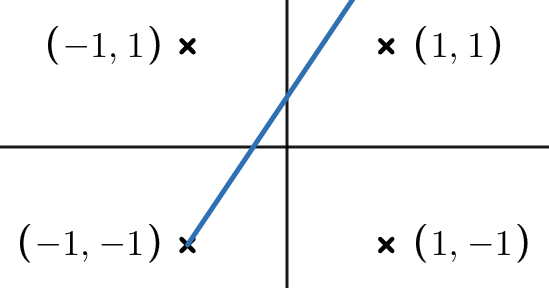
\includegraphics[width=0.5\linewidth]{Figures/DiscreteGradient.png}
    \caption{The optimal direction is indicated by the blue line, so the next state moves in that direction. The next state can be $(1,1)$ in parallel dynamics, whereas in sequential dynamics, it can be $(-1,1)$}
    \label{fig:discrete_gradient}
\end{figure}

\subsection{Sequential dynamics}
Many properties of the Ising model dynamics are obtained using sequential dynamics. In this part of the article, we will focus on this updating rule.

\begin{definition}[Lyapunov's function - \citet{Lyapunov}]
    \label{def:Lypunov}
    Given an autonomous dynamical system $\dot{x} = f(x)$ with equilibrium point $x_0$, a Lyapunov function is a function $V$ such that:
    \begin{itemize}[itemsep=2pt, topsep=10pt]
        \item $V(x) > 0$ with $x\neq x_0$
        \item $V(x_0) = 0$
        \item $\nabla V(x) \cdot f(x) \leq 0$
    \end{itemize}
    If $V$ exists then $x_0$ is stable for Lyapunov.\\ Remark: for a Lyapunov function it holds that $\dot{V}\left(x\right) \leq 0$
\end{definition}

\bigskip\noindent The dynamics of the neural network are a discretization of an autonomous dynamical system. In this subsection, we will refer to the function denoted by $L_{J,h}$ as a Lyapunov function, although this is not a rigorous definition. The following lemma defines this function and relates the interpretation in \cref{fig:discrete_gradient} to the Lyapunov function in \cref{def:Lypunov}.

\begin{lemma}[Decreasing function] \label{lemma:Lyap}
    Using Ising's model with sequential dynamics and interaction $J$ such that $J_{ii} \geq 0$ and $J_{ij}=J_{ji}$, the following function:
    \[
          L_{J,h}(\xi) = -\frac{1}{2} \sum_{ij} \xi_i J_{ij} \xi_j - \sum_{i} h_i \xi_i
    \]
    decreases over time: $L_{J,h}\left(\xi^{\text{new}}\right) \leq L_{J,h}\left(\xi\right)$.

    \begin{proof}
    \noindent Sequential dynamics can change only one value of the network so we can suppose that $i$ is the updated neuron: $\xi_k^{\text{new}} = \xi_k$ for all $k\neq i$.

    \noindent If $\xi_i^{\text{new}} = \xi_i$ there is not any difference, so now we assume $\xi_i^{\text{new}} = -\xi_i$ and study the variation of Lyapunov function $\Delta L_{J,h}$:
    \begin{align*}
         \Delta L_{J,h}\left(\xi,\xi^{\text{new}}\right) &= - \frac12 \sum_{k,l} J_{kl}\left(\xi_k^{\text{new}}\xi_l^{\text{new}} - \xi_k \xi_l\right) - \sum_l h_l \left(\xi_l^{\text{new}}-\xi_l\right) \\
         &\upeq{1} - \sum_{l \neq i} J_{il}\left(\xi_i^{\text{new}}\xi_l^{\text{new}} - \xi_i \xi_l\right) - (-2 h_i\xi_i) \\
         &= - \sum_{l \neq i} J_{il}\left(-\xi_i\xi_l - \xi_i \xi_l\right) - (-2 h_i\xi_i) = 2 \sum_l J_{il} \xi_i \xi_l + 2h_i \xi_i - J_{ii} \\
         &= 2 \xi_i \left( \sum_l J_{il} \xi_l + h_i \right) - J_{ii} \upeq{2} -2\left|\left( \sum_l J_{il} \xi_l +h_i \right)\right| - J_{ii} \leq 0
    \end{align*}
    In equivalence $1$ we used the symmetry of $J$ and $\xi,\xi^{\text{new}} = \pm1$.\\ In equivalence $2$ we used the update formula:
    \[
        \xi_i\left( \sum_l J_{il} \xi_l + h_i \right) = \xi_i\sgn\left[\sum_l J_{il} \xi_l +h_i \right]\left|\sum_l J_{il} \xi_l +h_i \right| = \xi_i\xi_i^{\text{new}}\left|\sum_l J_{il} \xi_l +h_i \right|
    \]
    \end{proof}
\end{lemma}

\begin{remark}[lower bound]
    We can see that the Lyapunov function is lower bounded:
\begin{align*}
    L_{J,h}(\xi) &= -\frac12 \sum_{i,j} \xi_iJ_{ij}\xi_j - \sum_i h_i\xi_i \\
    &\geq -\frac12 \sum_{i,j} J_{ij} - \sum_i h_i \geq -\frac{N^2}{2} |J| - N |h|
\end{align*}
where $|J| = \max_{i,j} |J_{ij}|$ and $|h| = \max_i |h_i|$.

\noindent Through the dynamic of the Ising's model, the value of the Lyapunov function decreases until it reaches a minimum $L^*$.
\end{remark}

\noindent The last step is to find a fixed point of the updating (in sequential dynamic) and to obtain the lower bound at it. In this way we know that the fixed point is stable for Lyapunov. The idea is to choose $J$ and $h$ such that the final configuration of the system is something meaningful. In particular, we want to store $P$ patterns $(x_1,...,x_P)$ in the network and given a starting point $\xi$ retrieve some pattern as the final point of the dynamics. Following this perspective we can interpret the value of the Lyapunov function as an energy function for the system that will evolve towards the minimum points.

\noindent We need to make these patterns the minimum points of the Lyapunov function to do this analysis. This problem can be solved using Hebb's rule:
\begin{definition}[Hebb's rule]
    \label{def:Heb}
    Given $P \leq N$ patterns $(x_1,\ldots,x_P)$ we define Hebbian interaction matrix as:
    \[
    J_{ij} = \frac1N (1 - \delta_{i,j}) \sum_{\mu=1}^P x^{\mu}_i x^{\mu}_j
    \]
\end{definition}
\begin{lemma}[Pattern as minimum points]
   \label{lemma:Heb}
   Let $J$ be made with the Hebbian rule using orthogonal patterns (i.e. $\sum_i x^{\mu}_i x^{\nu}_i =N \delta_{\mu,\nu}$ ), every pattern $x^{\mu}$ is a global minimum for the Lyapunov function with $h=0$.
   \begin{proof}
       \begin{align*}
            L_{J,h}(\xi) &= -\frac12 \sum_{i,j} \xi_i J_{ij} \xi_j  =
            -\frac12 \frac1N \sum_{i,j} (1 - \delta_{i,j}) \sum_{\mu} x^{\mu}_i x^{\mu}_j \xi_i \xi_j \\
            &= -\frac12\frac1N \sum_{i \neq j} \sum_{\mu} x^{\mu}_i x^{\mu}_j \xi_i \xi_j =
            \frac12P  -\frac12\frac1N \sum_{i,j} \sum_{\mu} x^{\mu}_i x^{\mu}_j \xi_i \xi_j = \\
            &= \frac{1}{2}P - \frac{1}{2}\sum_{\mu} \left( \frac{1}{\sqrt{N}} \sum_i x^{\mu}_i \xi_i \right)^2 \geq \frac{1}{2}(P - N) \upeq{1}  L_{J,h}(x^{\nu}) \quad \forall x^{\nu} \in (x_1,\ldots,x_P)
            \end{align*}
            the last inequality holds because of the orthogonality of the patterns with same euclidean norm $N$:
            \[
            \sum_{\mu} \left( \frac{1}{\sqrt{N}} \sum_i x^{\mu}_i \xi_i \right)^2 = \|\xi\|^2 \leq N
            \]
   \end{proof}
\end{lemma}

\subsection{Stochastic model}
With this framework we already use the network for pattern retrieval, but there are two main problems: the first is that the patterns are not always orthogonal, the second is that we can also retrieve a local minimum of the Lyapunov function, to overcome this problem we introduce the stochastic model.

\noindent Assume that $U^\star$ is not a deterministic threshold, and that we can express it in this way:
\[
    \forall{i}\left(U_i^\star\left(t\right) = U_i^\star - \frac12 T z_i\left(t\right)\right)
\]
with $z_i\left(t\right)\sim\mathcal{P}$ such that it's symmetric ($\implies\overline{z_i\left(t\right)}=0$) and $\overline{z_i\left(t\right)^2}=1$. The distribution function of $\mathcal{P}$ is denoted with $g\left(x\right)=\frac12 + \int_0^x\mathcal{P}\left(u\right)du$.

\noindent $T$ is called \textbf{temperature} and is not negative. The temperature controls the randomness of the process: $T=0$ implies a deterministic behaviour and as T increases, the behaviour tends to become increasingly random, approaching completely random behaviour in the limit as $T \to \infty$.

\begin{remark}
   We will use $g\left(x\right)=\frac12\left(1-\tanh\left(x\right)\right)$
\end{remark}

\begin{definition}[Stochastic sequential dynamics]
    \label{def:stocdyn}
    Consistent with the sequential dynamics of the deterministic process, we define the stochastic update using a non-deterministic threshold.

    \noindent Let $U_t\sim \textit{Unif}\left(\left[N\right]\right)$, for each component $i$ it holds that:
    \[ \xi_i^{t+1} \mathdef
    \begin{cases}
        \sgn\left[\phi_i(\xi^t) + Tz_i(t)\right] & \text{if }\;U_{t+1}=i \\
        \xi_i^t & \text{otherwise}
    \end{cases}
    \]
    remark: $z_i$ is a random variable for each $t$.
\end{definition}

\begin{lemma}[stochastic derivation]
    \label{lemma:stoch_der}
    Using an Ising model with sequential dynamics, we can formulate the following thesis:
    \[
        \mathbb{P}\left[\xi^{t+1}=\xi'\middle|\xi^t=\xi\right] =
        \frac{1}{N}\sum_i \frac{1}{2} (1 + \xi'_i \tanh(\beta \phi_i(\xi' )) \delta_{\xi,\xi'} + \frac{e^{-\beta \xi_i \phi_i(\xi)}}{2\cosh(\beta\phi_i(\xi))} \delta_{F_i(\xi),\xi'}
    \]
    where $F_i $ is the flip operator (it changes the sign of the $i^{\text{th}}$ component) and $\beta = \frac{1}{T}$
    \begin{proof}
    We can divide the proof in three cases:
    \begin{itemize}
        \item[i)] $\xi' = \xi$
        \begin{align*}
            &\mathbb{P}\left[\xi^{t+1}=\xi'\middle|\xi^t=\xi\right]
            = \mathbb{P}\left[\xi^{t+1}=\xi\middle|\xi^t=\xi\right]
            = \sum_i \mathbb{P}\left[\xi^{t+1}=\xi\middle|\xi^t=\xi, U_{t+1}=i\right]\mathbb{P}\left[U_{t+1}=i\right] \\
            &= \frac1N \sum_i \mathbb{P}\left[ \sgn\left[\phi_i(\xi^t) + Tz_i(t) \right] = \xi_i\middle|\xi^t=\xi, U_{t+1}=i\right]
            = \frac1N \sum_i \mathbb{P}\left[ \sgn\left[\phi_i(\xi) + Tz_i(t) \right] = \xi_i\right] \\
            &= \frac1N \sum_i \mathbb{P}\left[ \xi_i\left(\phi_i(\xi) + Tz_i\left(t\right) \right) \geq 0 \right]
            \upeq{1} \frac1N \sum_i \mathbb{P}\left[z_i(t) \geq - \beta \xi_i \phi_i\left(\xi\right) \right] \\
            &= \frac1N \sum_i \frac12 \left(1 + \xi_i \tanh\left(\beta \phi_i\left(\xi\right)\right)\right)
        \end{align*}
        In equivalence $1$ we used the relation $\xi_i z_i \sim z_i$ due to the symmetry

        \item[ii)] $\xi' = F_i(\xi)$
        \begin{align*}
            &\mathbb{P}\left[\xi^{t+1}=\xi'\middle|\xi^t=\xi\right]
            = \mathbb{P}\left[\xi^{t+1}=F_i(\xi)\middle|\xi^t=\xi\right] \\
            &= \mathbb{P}\left[\xi^{t+1}=F_i(\xi)\middle|\xi^t=\xi, U_{t+1}=i\right]\mathbb{P}\left[U_{t+1}=i\right] + \mathbb{P}\left[\xi^{t+1}=F_i(\xi)\middle|\xi^t=\xi, U_{t+1}\neq i\right]\mathbb{P}\left[U_{t+1}\neq i\right]\\
            &= \frac{1}{N} \mathbb{P}\left[ \sgn\left[\phi_i(\xi^t) + Tz_i(t) \right] = F_i(\xi)_i\middle| \xi^t=\xi, U_{t+1}=i\right] \\
            &= \frac{1}{N}  \mathbb{P}\left[ \xi_i\left(\phi_i(\xi^t) + Tz_i\left(t\right) \right) \leq 0 \right]
            = \frac{1}{N} \mathbb{P}\left[z_i(t) \leq - \beta \xi_i \phi_(\xi) \right] \\
            &= \frac{1}{2} \left(1 - \xi_i \tanh\left(\beta \phi_i\left(\xi \right)\right)\right) = \frac{e^{-\beta \xi_i \phi_i(\xi)}}{2\cosh(\beta\phi_i(\xi))}
        \end{align*}
        \item[iii)] otherwise\\
        Sequential dynamics can only change one neuron for each update so the probability is $0$.
    \end{itemize}

    \end{proof}
\end{lemma}

\paragraph{Markov chains} In \cref{lemma:stoch_der} we proved that only the last state established the new state. This condition defines a Markov chain over $\{-1,1\}^N$. Define $W_{\xi,\xi'}$ the probability to jump from $\xi$ in $\xi'$:
\[
    W_{\xi,\xi'} =
        \frac{1}{N}\sum_i \frac{1}{2} (1 + \xi'_i \tanh(\beta \phi_i(\xi' )) \delta_{\xi,\xi'} + \frac{e^{-\beta \xi \phi_i(\xi)}}{2\cosh(\beta\phi_i(\xi))} \delta_{F_i(\xi),\xi'}
\]
The matrix $W=\left(W_{\xi,\xi'}\right)_{\xi,\xi'}$ is the transition matrix of the Markov chain.

\begin{remark}
    Recall following properties:
    \begin{itemize}[itemsep=2pt, topsep=5pt]
        \item $\exists\tau\left(t\geq\tau\implies W^t > 0\right)$, so it is an ergodic Markov chain. So there exists a unique invariant distribution $p_{\infty}$ to which the process will converges form any initial state.
        \item If $\forall \xi,\xi'\left(p(\xi) W_{\xi,\xi'} = p(\xi') W_{\xi'\xi}\right)$ then $p$ is an invariant distribution. The equivalence is called \textbf{detailed balance}.
    \end{itemize}
\end{remark}

\noindent We use stochastic dynamics to escape from non-optimal minima. Now we study a limit probability of the state of the neural network using weights $J$ similar to  \cref{def:Heb}. But before addressing the following theorem let us recall this lemma from graph theory.
\begin{lemma}
    \label{lemma:combinatorics}
    Let $G$ graph with vertices $V$ and oriented edges $E$ such that a vertex connected with all vertices exists, called $O$. Each edge $\vec{e}$ has a value $c(\vec{e})$ and $c(-\vec{e}) = -c(\vec{e})$ (it is called '\textit{flux}'). The function $K:V\to\mathbb{R}$ (called potential) is such that $K(v)-K(w)=c(\vec{vw})$ exists if and only for each cycle $\vec{e_1},\ldots,\vec{e_n}$ holds $\sum c(\vec{e_k}) = 0$ (flow conservation).

    \begin{proof}
        If $K$ exists, then it's clear that the summation of values over a cycle is $0$.

        \noindent If flow conservation holds, then for each vertices $v$ we can find a path $\vec{e_1},\ldots,\vec{e_n}$ to $O$ from $v$ with vertices $O=v_0,\ldots,v_n=v$, so:
        \[
        K(v)-K(O) = \sum K(v_{i+1}) - K(v_{i})
        \]
        remark: potential exists at less than a constant.
    \end{proof}
\end{lemma}

\begin{theorem}[Invariant measure] \label{teo:Inv_Mea}
    In a sequential stochastic dynamic without self-interactions, i.e. $J_{ii}=0$, detailed balanced is equivalent to symmetric interactions:
    \[
    J_{ij}= J_{ji} \iff p_\infty(\xi) W_{\xi\xi'} = p_\infty(\xi') W_{\xi'\xi} \quad \forall \xi,\xi'
    \]
    Furthermore, the stationary distribution is:
    \[
    p_{\infty}(\xi) \propto e^{-\beta \mathcal{H}_{J,h}(\xi)}
    \]
    where $\mathcal{H}_{J,h} =  -\frac{1}{2} \sum_{i,j} \xi_i J_{ij} \xi_j - \sum_{i} h_i \xi_i$ (called Hamiltonian function).
    \begin{proof}
        We know that if $p$ verifies the detailed balance and $p$ is a distribution, then $p_\infty=p$. So we are going to start by finding an explicit form of a distribution that verifies detailed balance. We are going to prove that this distribution exists if $J$ is symmetric, and then the opposite (only if $J$ is symmetric).

        \bigskip\noindent At the moment, we are rewriting detailed balance in a simple form. \\ If $\xi'=\xi$ or $\xi'\neq\xi \land \forall i\left(\xi' \neq F_i(\xi)\right)$ the detailed balance holds trivially because we get $0=0$. For each $\xi,\xi'$ such that $\exists i\left(\xi' = F_i(\xi)\right)$, we want to express the detailed balance in a simpler form. Using \cref{lemma:stoch_der}:
        \[
            p_{\infty}(\xi) \frac{e^{-\beta \xi_i \phi_i(\xi)}}{2\cosh(\beta\phi_i(\xi))} = p_{\infty}(\xi') \frac{e^{-\beta \xi'_i \phi_i(\xi')}}{2\cosh(\beta\phi_i(\xi'))}
        \]
        We remark that there's no self-interaction, so:
        \[
            \phi_i(\xi) = \sum_j J_{ij}\xi_j+h_i = \sum_{j\neq i} J_{ij}\xi_j + h_i = \sum_{j\neq i} J_{ij}\xi'_j + h_i = \sum_{j} J_{ij}\xi'_j + h_i = \phi_i ( \xi')
        \]
        This gives us an equivalent form of detailed balance sheet:
        \begin{align}
            \label{tmp:1}
            &\forall \xi,\xi'\left(p_\infty(\xi) W_{\xi\xi'} = p_\infty(\xi') W_{\xi'\xi}\right) \\
            &\iff \forall \xi,\xi',i\left(\xi' = F_i(\xi) \implies p_{\infty}(\xi) e^{-\beta \xi_i \phi_i(\xi)} = p_{\infty}(\xi') e^{-\beta \xi'_i \phi_i(\xi')} \right) \nonumber
        \end{align}

        \bigskip\noindent Now let's try to find a distribution $p$ that verifies the detailed balance. We know that the distribution $p_\infty$ is positive over all states, so our target distribution has to be positive over all states as well. We can write $p$ in exponential form: $p\left(\xi\right)=\exp\left(-\beta K(\xi)\right)$. This simplifies the equivalent form in \cref{tmp:1}.

        \noindent Using \cref{tmp:1}, we can verify detailed balance only over the couples $\xi,\xi'$ such that $\exists i\left(\xi'=F_i\left(\xi\right)\right)$. Simplifying:
        \begin{align*}
            &K(\xi) + \xi_i\phi_i(\xi) = K(\xi') + \xi'_i\phi_i(\xi') \\
            &K(\xi')-K(\xi) = 2\xi_i\phi_i(\xi) = 2\xi_i\left(\sum_l J_{il}\xi_l + h_i\right)
        \end{align*}
        Using \cref{lemma:combinatorics}, it is possible to find an explicit form of $K$ if and only if $2\xi_i\left(\sum_l J_{il}\xi_l + h_i\right)$ is a flux that verifies the flow conservation.

        \noindent We can express the flow conservation with a simpler and equivalent condition.

        \noindent Let $i,j$ be different indices, get a path $\mathcal{P}_1=\left(v,F_i(v),F_j(F_i(v))\right)$, we want that the flux over $\mathcal{P}_1$ to be the same flux over $\mathcal{P}_2 = \left(v,F_j(v),F_i(F_j(v))\right)$:
        \begin{align*}
            \text{flux}\left(\mathcal{P}_1\right) &= 2v_i\left(\sum_l J_{il}v_l + h_i\right) + 2F_i(v)_j\left(\sum_l J_{jl}F_i(v)_l + h_j\right) \\
            &= 2v_i\left(\sum_l J_{il}v_l + h_i\right) + 2v_j\left(\sum_l J_{jl}v_l + h_j - 2J_{ji}v_i\right) \\
            &= 2v_i\left(\sum_l J_{il}v_l + h_i\right) + 2v_j\left(\sum_l J_{jl}v_l + h_j\right) - 2J_{ji}v_jv_i \\
            \text{flux}\left(\mathcal{P}_2\right) &= 2v_j\left(\sum_l J_{jl}v_l + h_i\right) + 2F_j(v)_i\left(\sum_l J_{il}F_j(v)_l + h_i\right) \\
            &= 2v_j\left(\sum_l J_{jl}v_l + h_j\right) + 2v_i\left(\sum_l J_{il}v_l + h_i - 2J_{ij}v_j\right) \\
            &= 2v_j\left(\sum_l J_{jl}v_l + h_j\right) + 2v_i\left(\sum_l J_{il}v_l + h_i\right) - 2J_{ij}v_iv_j
        \end{align*}
        so $\text{flux}\left(\mathcal{P}_1\right) = \text{flux}\left(\mathcal{P}_2\right) \iff J_{ij}=J_{ji}$.

        \noindent The flow does not change when we commute $2$ flips. In a cycle we know that if we have a flip $F_i$ then there is another $F_i$. Using commutation we can remove all flips and so the flux is conservative.

         \noindent We prove that there is a potential at less than a constant, and in order to get a distribution from $K$, it's possible to set a particular potential $K(\xi) + \const$ such that $p$ is a distribution. Now we know that the thesis is true, so we can compute $K$ to prove that $p_{\infty}(\xi) \propto e^{-\beta \mathcal{H}_{J,h}(\xi)}$.

        \noindent Seeing that $K(\xi')-K(\xi) = 2\xi_i(\sum_l J_{il}\xi_l + h_i)$ we recognize the result in \cref{lemma:Lyap}:\\ $K(\xi') - K(\xi) = \Delta L_{J,h}(\xi,\xi')$

        \noindent So a good option for the potential $K$ is:
        \[
            K(\xi) = -\frac12\sum_{ij}\xi_iJ_{ij}\xi_j - \sum_i h_i\xi_i + \const = \mathcal{H}_{J,h}(\xi) + \const
        \]
    \end{proof}
\end{theorem}

\section{Statistical mechanics perspective}
According to \cref{teo:Inv_Mea}, there is a connection between the dynamics of the network and spin models studied in statistical mechanics, since the state of a neuron can be associated with the alignment of an atom in a magnetic field, or its spin. Statistical mechanics, a branch of physics, connects the individual properties of atoms or molecules to macroscopic observable quantities such as temperature and pressure. This framework provides insight into how the collective behavior of many particles gives rise to the thermodynamic properties we observe. Using this approach, we can analyze how the behavior of the system changes in response to changes in its parameters. The key idea is to interpret the state of the system as a mixture of pure states - a probability distribution over these pure states - and to identify the configuration that minimizes a given energy function. Another essential aspect is to determine specific order parameters on which the probability distribution depends; by analyzing these, we can gain insight into the behavior of the entire system.

\begin{definition}
	\label{def:gibbs_stat}
	According to statistical mechanics, we can define a state of a system $\rho$ as a convex combination of the set of pure states $\{\rho^1,\ldots,\rho^{\mathcal{N}} \}$\\
	Given a state $\rho$, we define the following quantities:
	\begin{itemize}
		\item[i)] $U(E,\rho) = \sum_i \rho_i E_i$ \quad\textbf{internal energy}
		\item[ii)] $S(\rho) = -K_B \sum_i \rho_i \log(\rho_i) $ \quad \textbf{Gibbs entropy}
		\item[iii)] $ f(E,\rho,T) = U(E,\rho) - T S(\rho) $ \quad \textbf{free energy}
	\end{itemize}
\end{definition}
\begin{definition}[Gibbs distribution]
    \label{def:GibbsDist}
    The limit distribution given in \cref{teo:Inv_Mea} plays a key role in statistical mechanics. In this setting we can rephrase it as Gibbs distribution: \\
    \[
    \rho_{\beta}(\xi) = \frac{e^{-\frac{\beta E(\xi)}{K_B}}}{Z_{\beta}}
    \]
    where: $Z_\beta = \sum_\xi e^{-\frac{\beta E(\xi)}{K_B}} $ is the normalization factor called \textbf{partition function}.

    \bigskip\noindent In the context of neural networks:
    \begin{itemize}
       \item $E(\xi)=\mathcal{H}_{J,h}(\xi)$ is the energy of the neural network.
       \item $K_B=1$ is a taken factor.
    \end{itemize}
\end{definition}

\noindent The role of this distribution is given by the following theorem:
\begin{theorem}[Gibbs distribution]
     \label{teo:Gibbs}
     The Gibbs distribution is the state $\rho$ where the free energy reaches its minimum, this point is called thermodynamic equilibrium.
     \[
      \inf_\rho f(E,\rho,T) = f(E,\bar{\rho},T) = -K T \log(\bar{Z})
     \]
    where $\bar{\rho}$ is the Gibbs distribution
    \begin{proof}
        The free energy is a convex function with respect to $\rho$ because the energy is affine and the Gibbs entropy is concave, so we can find its minimum by finding the point where $\delta f = 0$ $\forall \rho$ variations.
        Hence we obtain:
        \[
        \begin{cases}
            \delta f = \sum_i E_i\delta\rho_i  + KT(\log(\rho_i)+1)\delta\rho_i \upeq{1} \sum_i (E_i + KT\log(\rho_i))\delta\rho_i = 0 \\
            \sum_i \delta\rho_i = 0
        \end{cases}
        \]
        In equivalence $1$ we use the second equation.

        \noindent From the first equation we can state that $E_i + KT\log(\rho_i)$ must not depend on $i$ because the system must hold for any variation. So we can say that if $\bar{\rho}$ exists then:
        \[
        E_i + KT\log(\bar{\rho_i}) = \bar{F}
        \]
        from which we get $\bar{\rho_i}$, we have:
        \[
        \bar{\rho}_i = e^{-\frac{E_i-\bar{F}}{KT}}
        \]
        The constant $\bar{F}$ must be taken to satisfy:
        \[
         1=\sum_i \bar{\rho}_i = \sum_i e^{-\frac{E_i-\bar{F}}{KT}} = e^{\frac{\bar{F}}{KT}}\sum_i e^{-\frac{E_i}{KT}}
        \]
        \noindent Using the definition of free energy and the formula for $\bar{\rho}$ we obtain:
        \begin{equation}
            f(E,\bar{\rho},T) = \bar{F}e^{\frac{\bar{F}}{KT}}\sum_i e^{-\frac{E_i}{KT}} = \bar{F}
        \end{equation}
        We can state that $\bar{Z} = e^{-\frac{\bar{F}}{KT}}$.
    \end{proof}
\end{theorem}

\bigskip\noindent We introduced noise to escape unwanted local minima, but in this way it is not possible to assume that the sequence converges to ideal states. So we found the limit distribution and observed that it is the Gibbs distribution (see \cref{teo:Inv_Mea}).

\noindent As the sequential deterministic dynamics reduces the Lyapunov function (see \cref{lemma:Lyap}), the sequential stochastic dynamics reduces the free energy. However, the convergence is towards the optimal density (see \cref{teo:Gibbs}).

\subsection{Curie-Weiss model}
To introduce the way of working of statistical mechanics, we begin with an analysis of the Curie-Weiss model.
\begin{definition}[Curie-Weiss model]
	The Curie-Weiss model is an Ising model in which the Hamiltonian function is:
	\[
	\mathcal{H}_{N,J,h}(\xi) = - \sum_{i\neq j} \frac{J}{2} \xi_i \xi_j - h \sum_i \xi_i
	\]
	Note: This is a special case where $J_{ii}=0$, $J$ symmetric and $J_{ij}$ is constant where $i\neq j$.
\end{definition}
This type of model is called a mean field model because each neuron interacts with all the others in the same way. The goal of the analysis here is to understand the behavior of the magnetization.
\begin{definition}[magnetization]
	Given a state $\xi$ we call the magnetization the quantity:
	\[
	m_N(\xi) = \frac{1}{N} \sum_i \xi_i
	\]
\end{definition}
The magnetization is what we call an observable quantity because it depends on the state of all the neurons, not just one. An important observation is that we can write the Hamiltonian as a function of the magnetization as:
\[
	\mathcal{H}_{N,J,h}(\xi) = - \frac{NJ}{2} m_N(\xi)^2 - h N m_N(\xi)
\]
We know thanks to the \cref{teo:Gibbs} that the distribution that minimizes the free energy is the observed one, but we don't know anything about the magnetization, so our goal is to understand how it is effected by the temperature, at least when $N$ is very large. Taking $N \to \infty$ is a key concept in statistical mechanics and it is called thermodynamic limit (TDL) it allows us to simplify some calculations by removing the dependence from the size of the model. To calculate the thermodynamic limit, we need to recall and introduce some quantities:
\begin{definition}[Curie-Weiss quantities]
\label{def:CWqt}
We define quantities for Curie - Weiss model:
    \begin{itemize}
        \item $\rho_{N,\beta,J,h}(\xi) =\frac{ e^{-\beta \mathcal{H}_{N,J,h}(\xi)}}{Z_{N,\beta,J,h}} $ \quad \textbf{equilibrium distribution}
        \item $Z_{N,\beta,J,h} $ \quad \textbf{partition function}
        \item $F_{N,\beta,J,h} = -\frac{1}{\beta } \log(Z_{N,\beta,J,h}) $ \quad \textbf{free energy}
        \item $f_{N,\beta,J,h} = -\frac{1}{\beta N} \log(Z_{N,\beta,J,h}) $ \quad \textbf{intensive free energy}
        \item $f_{\beta,J,h} = \lim_{N \to \infty} f_{N,\beta,J,h}$ \quad \textbf{intensive free energy in TDL}
    \end{itemize}

	\bigskip\noindent Note: These definitions are addressed with definitions in \cref{def:gibbs_stat} using the Gibbs distribution $\bar{\rho}$.
\end{definition}
Now we are ready to analyze the Curie-Weiss model.

\noindent First, we will try to understand the probability distribution of the magnetization when the states follow the equilibrium distribution (\cref{def:GibbsDist}):
\[
\rho_{N,\beta,J,h}(m) \mathdef \mathbb{P}_{\xi\sim\bar{\rho}}\left[m_N(\xi) = m\right] = \sum_{\xi}  \rho_{N,\beta,J,h}(\xi) \delta(m_N(\xi) = m )
\]
This measure is called \textbf{coarse grained measure} and our goal is to understand how it relates to the equilibrium measure in the TDL.\\
We also introduce the coarse-grained partition function, which is
\[
Z_{N,\beta,J,h}(m) \mathdef \sum_{\xi} e^{-\beta \mathcal{H}_{N,J,h}(\xi)} \delta(m_N(\xi) = m )
\]
\begin{definition}[coarse grained measure] We will continue these definitions with other coarse-grained partition functions:
    \begin{itemize}
        \item $\rho_{N,\beta,J,h}(m) = \sum_{\xi}  \rho_{N,\beta,J,h}(\xi) \delta(m_N(\xi) = m ) $ \quad \textbf{probability magnetisation}
        \item $Z_{N,\beta,J,h}(m) = \sum_{\xi} e^{-\beta \mathcal{H}_{N,J,h}(\xi)}  \delta(m_N(\xi) = m ) $ \quad \textbf{partition function}
        \item $F_{N,\beta,J,h}(m) = -\frac{1}{\beta } \log(Z_{N,\beta,J,h}(m)) $ \quad \textbf{free energy}
        \item $f_{N,\beta,J,h}(m) = -\frac{1}{\beta N} \log(Z_{N,\beta,J,h}(m)) $ \quad \textbf{intensive free energy}
        \item $f_{\beta,J,h}(m) = \lim_{N \to \infty} f_{N,\beta,J,h}(m)$ \quad \textbf{intensive free energy in TDL}
\end{itemize}
\end{definition}

\begin{proposition}
    Using this formalism we can express the probability of the magnetization from the intensive free energy in TDL:
    \begin{align}
        \rho_{N,\beta,J,h}(m) &= \sum_{\xi}\frac{ e^{-\beta \mathcal{H}_{N,J,h}(\xi)}  \delta\left(m_N(\xi)
        = m\right)}{Z_{N,\beta,J,h}}
        = \frac{Z_{N,\beta,J,h}(m)}{Z_{N,\beta,J,h}} \nonumber \\
        &= \frac{\exp\left(\frac{\beta}{\beta}\log\left(Z_{N,\beta,J,h}\left(m\right)\right)\right)}{\exp\left(\frac{\beta}{\beta}\log\left(Z_{N,\beta,J,h}\right)\right)}
        = \frac{\exp\left(-\beta F_{N,\beta,J,h}(m)\right)}{\exp\left(-\beta F_{N,\beta,J,h}\right)}
        = e^{-\beta(F_{N,\beta,J,h}(m)-F_{N,\beta,J,h})} \nonumber \\
        &= e^{-\beta N \left(f_{N,\beta,J,h}(m)-f_{N,\beta,J,h}\right)} \label{eq:Z_m_sum}
    \end{align}
\end{proposition}
\begin{remark}
    In this way we can calculate the initial definitions in \cref{def:CWqt} in terms of intensive free energy in TDL:
    \begin{align}
        Z_{N,\beta,J,h} &= \sum_\xi \rho_{N,\beta,J,h}(\xi) = \sum_m \sum_\xi \rho_{N,\beta,J,h}(\xi)  \delta(m_N(\xi) = m ) \nonumber \\
        &= \sum_m  Z_{N,\beta,J,h}(m) = \sum_m e^{-\beta N f_{N,\beta,J,h}(m)}
    \end{align}
\end{remark}

\noindent This formulation suggests that the terms that most influence the partition function are those where the value of $f_{N,\beta,J,h}(m)$ is minimized. Moreover, if $f_{\beta,J,h}(m)$ has a minimum in $m^*$, we can state for the thermodynamic limit, using the Taylor expansion for $f_{\beta,J,h}(m)$, that
\begin{align*}
    \lim_{N\to\infty}Z_{N,\beta,J,h} &\upeq{1}  \lim_{N\to\infty}\sum_m e^{-\beta N f_{N,\beta,J,h}(m)} = \lim_{N\to\infty} \int_{-\infty}^{+\infty}  e^{-\beta N f_{\beta,J,h}(m)}dm \\
    &=\lim_{N\to\infty} \int_{-\infty}^{+\infty} e^{-\beta N\left(f_{\beta,J,h}(m^*) + \frac{f''_{\beta,J,h}(m^*)(m-m^*)^2}{2} \right)}dm\\
    &= \lim_{N\to\infty}e^{-\beta N f_{\beta,J,h}(m^*) } \sqrt{\frac{2\pi}{N\beta f''_{\beta,J,h}(m^*)}}
\end{align*}
Where in the equivalence $1$ we used a similar conclusion of \cref{eq:Z_m_sum}, using this relation within the definition of the intensive free energy in TDL we get:
\begin{align*}
    f_{\beta,J,h} &= \lim_{N \to \infty}  -\frac{1}{\beta N} \log(Z_{N,\beta,J,h})  \\
    &= \lim_{N \to \infty}  -\frac{1}{\beta N} \log\left(e^{-\beta N f_{\beta,J,h}(m^*) } \sqrt{\frac{2\pi}{N\beta f''_{\beta,J,h}(m^*)}} \right)\\
    &=  \lim_{N \to \infty} -\frac{-\beta N  f_{\beta,J,h}(m^*)}{\beta N}  -\frac{\log\left(\sqrt{\frac{2\pi}{N\beta f''_{\beta,J,h}(m^*)}} \right)}{\beta N}\\
    &=  \lim_{N \to \infty} f_{\beta,J,h}(m^*) =  f_{\beta,J,h}(m^*)
\end{align*}
So if we can find the minima of the intensive free energy for each $N$ ($m^\star_N$) and then we would like to be able to compute all minima $m^\star$ and thus the intensive free energy for TDL.

\bigskip\noindent From \cref{teo:Gibbs} we know that we can express intense free energy as
\[
     f_{N,\beta,J,h}(m) = \frac{E_{N,\beta,J,h}(\rho_{N,\beta,J,h}(m)) - T S(\rho_{N,\beta,J,h}(m))}{N}
\]
We consider only the configuration with a fixed magnetization, so the energy is constant and the distribution is uniform over the number of possible configurations, which allows us to say:
\[
    f_{N,\beta,J,h}(m) = \frac{- \frac{NJ}{2} m^2 - h N m}{N} - T \frac{S(\text{Unif}\left[\Omega_N(m)\right]))}{N} = - \frac{J}{2} m^2 - h  m +
    T \frac{\log(\Omega_N(m))}{N}
\]
where $\Omega_N(m) = \sum_\xi \delta(m(\xi)-m)$ is the number of possible configurations.

\noindent In the TDL we get
\begin{align*}
	f_{\beta,J,h}(m) =& \lim_{N\to \infty} f_{N,\beta,J,h}(m) = - \frac{J}{2} m^2 - h m + \lim_{N\to \infty} T \frac{\log(\Omega_N(m))}{N}\\ =& - \frac{J}{2} m^2 - h m + T\left[\frac{1+m}{2} \log\left(\frac{1+m}{2} \right) + \frac{1-m}{2} \log\left(\frac{1-m}{2} \right) \right]
\end{align*}
We are interested in finding the minimum so that we can take the derivative:
\[
f'_{\beta,J,h}(m) = -J m -h + T \left[\frac12 \log\left(\frac{1+m}{1-m} \right) \right] =
-J m -h + T \tanh^{-1}(m)
\]
So stationary points are characterized by the following equation:
\begin{equation}
	\label{eq:Sel_const_CW}
	m^* = \tanh(\beta (Jm^* + h))
\end{equation}
This relation is called the self-consistent equation for the Curie-Weiss model and we can't solve it analytically. We will analyze it when $h=0$ to understand where the minimum of the free energy is. \\
The first observation is that $m^*= 0$ is always a solution and we can find the solution graphically. In a Cartesian graph with the axis $x,y$ we draw the line $\left\{(x,y) \middle| y = x\right\}$ and the function $\left\{(x,y)\middle | y = \tanh(\beta (Jm^*)\right\}$. \\
\begin{figure}[!ht]
    \centering
    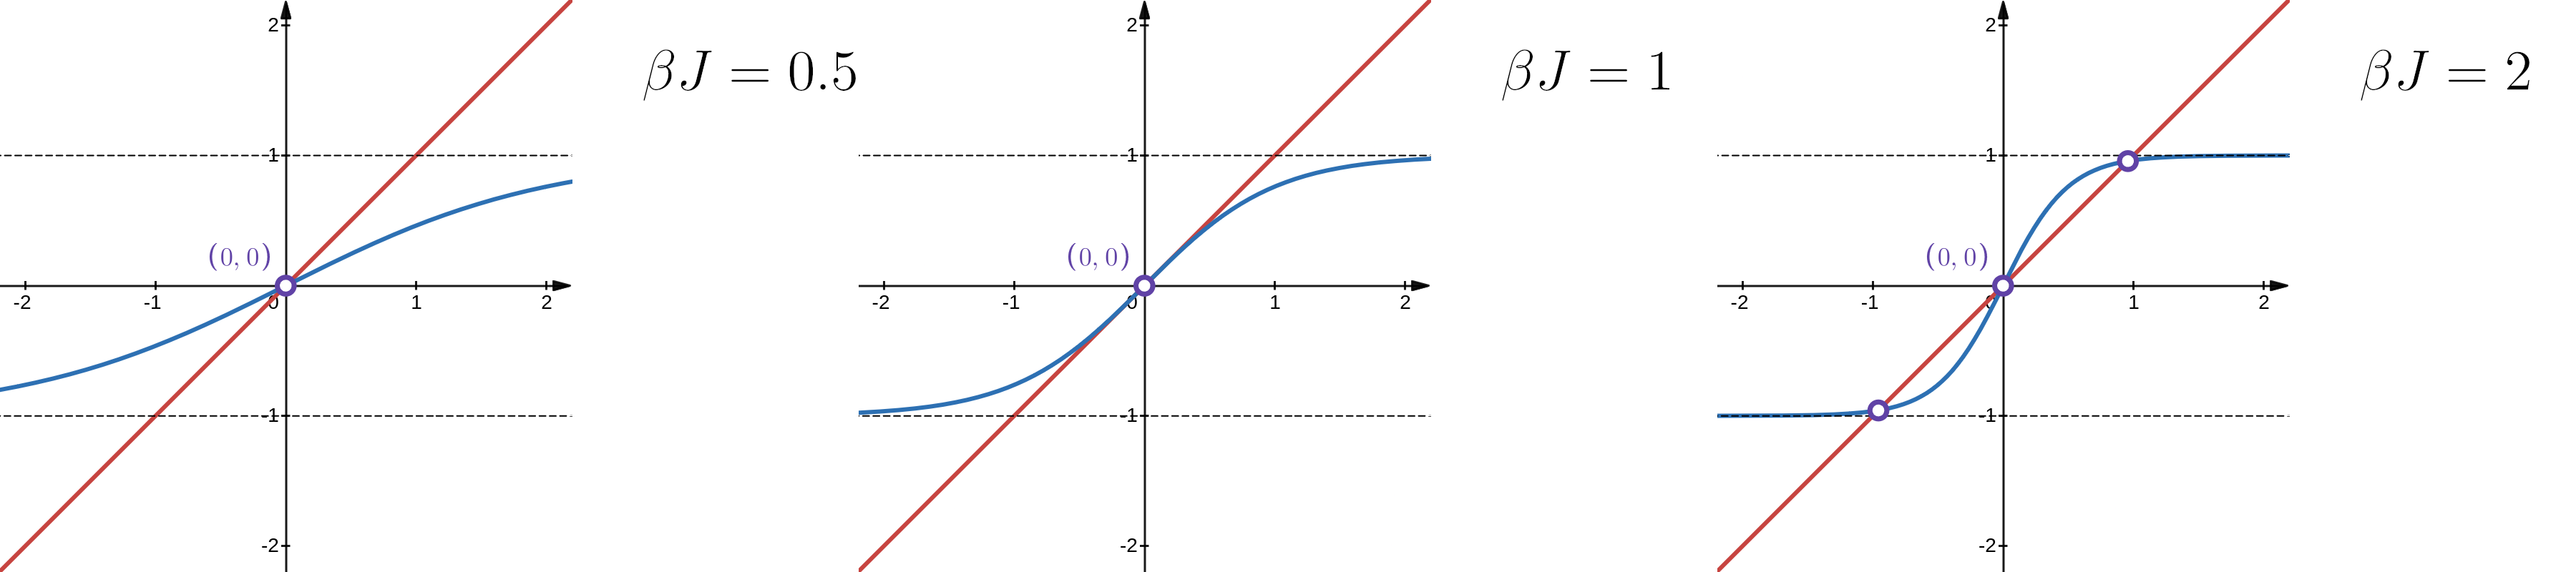
\includegraphics[width=1.0\linewidth]{Figures/3graphs.png}
\end{figure}
\bigskip\noindent We want to understand when the \cref{eq:Sel_const_CW} has one solution and when it has three solutions. To do this, we will analyze the derivative of $\tanh(\beta (Jm)$ in zero:
\[
   \frac{d\tanh(\beta Jm)}{dm}\bigg|_{m=0} = (1- \tanh^2(\beta Jm))\beta J \bigg|_{m=0} = \beta J
\]
From this we can see that the equation has one solution if $\beta J \leq 1$ and three solutions if $\beta J> 1$. \\
Now, from the graph of the free energy in both cases, we can see that $m^*= 0$ is a minimum if $\beta J \leq 1$ and that the positive and negative solutions are minima if $\beta J > 1$.\\
\begin{figure}[!ht]
    \centering
    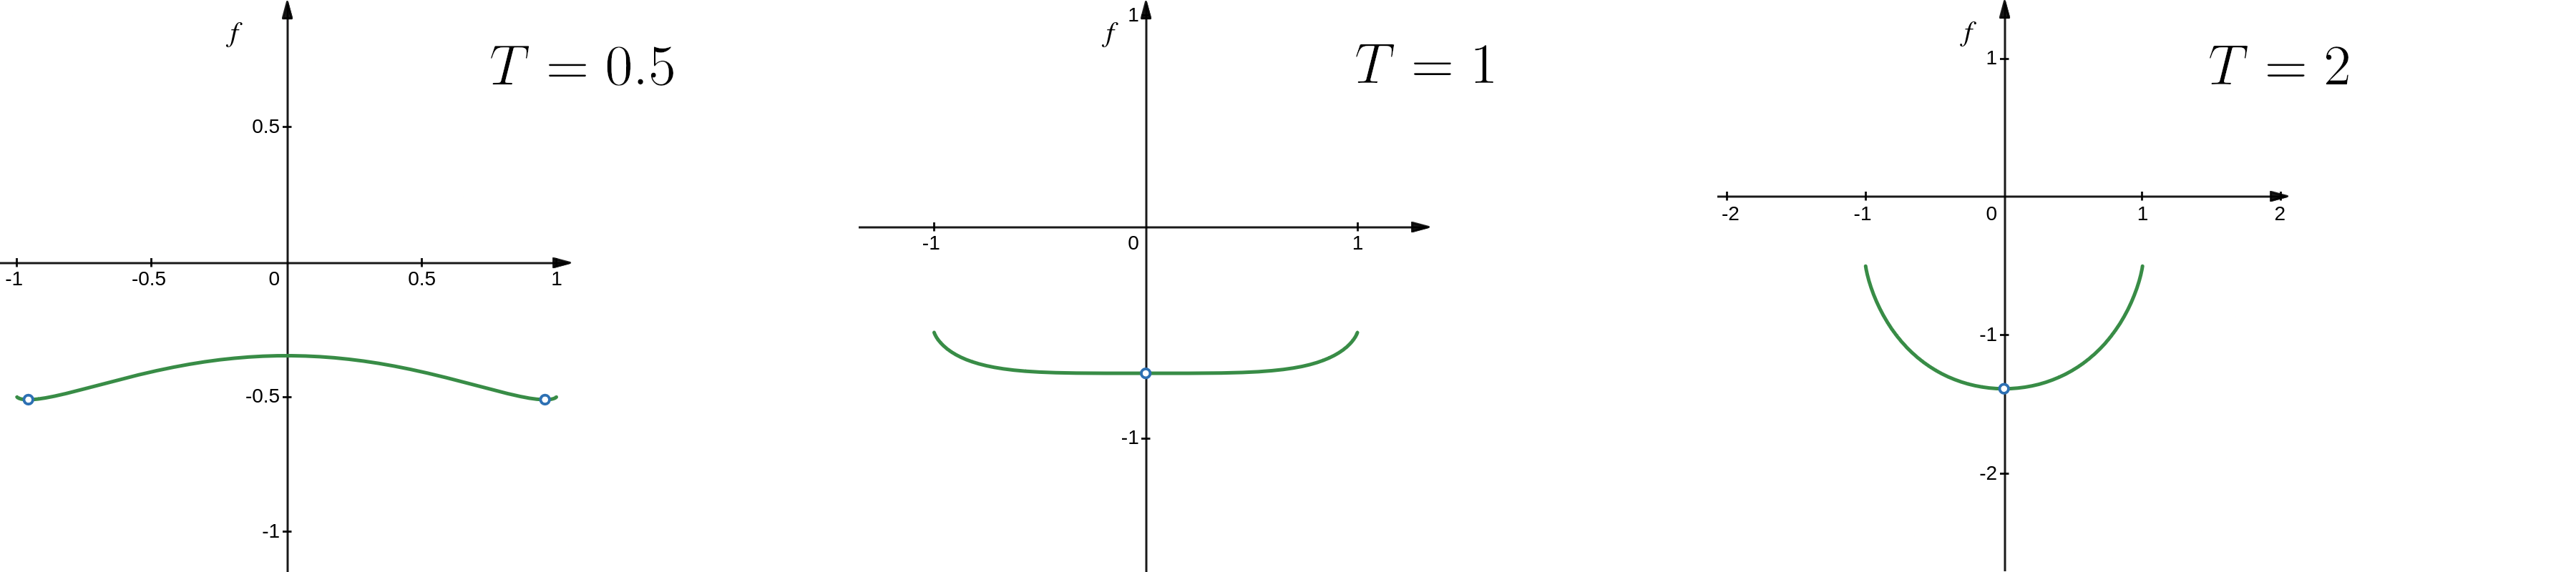
\includegraphics[width=1.0\linewidth]{Figures/3graphsE.png}
\end{figure}

The behavior of the system is completely different in the two cases divided by the critical temperature $T_c = J$, in fact for temperatures above $T_c$ randomness prevails and there are only disordered states, instead for temperatures lower than $T_c$ ordered states appear.  \\
Now we want to analyze the magnetization as a function of temperature to understand its behavior near the critical temperature.

\noindent To do this we will use the Taylor expansion of the hyperbolic tangent inside the \cref{eq:Sel_const_CW}:
\[
    m = \beta J m - \frac13 (\beta J m )^3 + o(m^5)
\]
Ignoring the higher order terms, we can find the solutions as follows:
\[
 m^* = \pm \sqrt{\frac{3(\beta J - 1)}{(\beta J)^3}} = \pm \sqrt{\frac{3(T_c-T)}{T_c (\beta J)^2}} \sim \sqrt{T_c-T}
\]
So we can conclude that the solution can be represented as a continuous function with a discontinuous derivative. \\ From this model we can understand two key concepts of statistical mechanics:
\begin{itemize}
	\item \textbf{Phase transition}\\
	We have seen that the magnetization can be written as a function of temperature and that this function has a
	discontinuous derivative. This phenomenon suggests that the model is in a completely different state depending on the temperature, just as different materials can be gas, solid and liquid. In statistical mechanics this type of behavior is called a phase transition and it is associated with a discontinuity of a derivative of the free energy.
	\item \textbf{Ergodicity breaking}\\
	In the previous setting we noticed that the Markov chain representing the dynamics of the model is ergodic, so it is possible to replace the space average of a quantity with infinite time average along the trajectory for any starting configuration instead in the TDL different starting point gives different result if the temperature is less than the critical temperature.
	This is only possible in TDL and makes the system no longer invariant to its symmetries (in CW a symmetry is given by flipping all neurons). This is something we want to transport into a neural network to get different results with different initial conditions.
\end{itemize}
The last question about the Curie-Weiss model is how it relates to the neural network we defined previously. To understand this connection, we consider a network with a single stored pattern $x$, $h=0$ and the interaction matrix $J$ built with \cref{def:Heb}. We get the following Hamiltonian
\[
\mathcal{H}_{N,J}(\xi) = - \sum_{i,j} J_{i,j} \xi_i \xi_j = - \frac{1}{N} \sum_{i\neq j} (\xi_i x_i)(\xi_j x_j) = - N m_{N,x}(\xi)^2
\]
where $m_{N,x}(\xi) = \frac{1}{N} \sum_i \xi_i x_i $ \quad \textbf{Mattis magnetization}\\
So it is equivalent to a Curie-Weiss model where $J = 2$.\\
Given an initial state, we can use as output the Mattis magnetization after a sufficient number of updates. We can affirm that with a large enough number of neurons (so we can use TDL as a good approximation) and a low temperature, the system will evolve to show a magnetization close to the chosen pattern. It is important to note that there are two main attractors in this type of system, one related to the actual pattern ($m_{N,x}(\xi) \approx 1$) and the other with its negative ($m_{N,x}(\xi) \approx -1$), so this simple network gives as output the pattern or its negative, depending on which is "closer" to the initial configuration.
\subsection{Hopfield model}
In the previous pages we analyzed a network that stores one pattern, now we want to understand networks with more patterns, so we try again to express the Hamiltonian as a function of some order parameter.
\begin{definition}[Mattis magnetizzation] \label{def:mattis_mgn}
Given the patterns $(x^1,\ldots,x^P)$ and a state $\xi$ we define:
\[
    m_{N,\mu}(\xi) = \frac{1}{N} \sum_i  \xi_i x^\mu_i \quad \forall \mu \in \{1,\ldots,P\}
\]
\end{definition}
This definition allows us to write the Hamiltonian with $J$ defined by the Hebb's rule (see \cref{def:Heb}) as:
\[
    \mathcal{H}_{N,X}(\xi)  = \frac12 \sum_{i,j} \frac1N (1 - \delta_{i,j}) \sum_{\mu=1}^P x^{\mu}_i x^{\mu}_j \xi_i \xi_j =
    -\frac{N}{2} \sum_\mu  m_{N,\mu}(\xi)^2
\]
As we defined before $P \leq N$ and $X \in \mathbb{R}^{N \times P}$ is the design matrix. As before we are interested in the analysis of the system in the TDL and we can have two cases:
\begin{itemize}
    \item \textbf{low load regime} where $\lim_{N\to\infty} \frac{P}{N} = 0$
    \item \textbf{high load regime} where $\lim_{N\to\infty} \frac{P}{N} > 0$
\end{itemize}
We will analyze the low load regime. We already know that the free energy can be expressed as the logarithm of the partition function, but with this method we do not remove the dependence of the free energy on the patterns $X$. To remove this dependence we need to define the concept of quenched free energy:
\begin{definition}[Quenched free energy]
We define the quenched free energy as the average over all possible pattern realizations of the free energy:
\begin{itemize}
    \item $Z_{N,\beta,X} = \sum_\xi e^{-\beta\mathcal{H}_{N,X}\left(\xi\right)}$ \textbf{partition function}
    \item $f_{N,\beta,X} = -\frac{1}{N\beta}\log\left(Z_{N,\beta,X}\right)$ \textbf{intensive free energy}
    \item $f_{\beta,X} = \lim_{N\to\infty} f_{N,\beta,X}$
    \item $f^Q_{N,\beta} = \mathbb{E}\left[f_{N,\beta,X}\right] = -\frac{1}{\beta N} \frac{1}{2^{N\times P}}\sum_{X \in \mathbb{R}^{N \times P}}\log( Z_{N,\beta,X}) $
    \quad \textbf{intensive quenched free energy}
    \item $f^Q_{\beta}= \lim_{N \to \infty} f^Q_{N,\beta}  $ \quad \textbf{intensive quenched free energy in TDL}
\end{itemize}
\end{definition}
In the previous definition it is important that the averaging is done before the TDL, in fact it is not true that we can invert these operations.\\
\begin{remark}
    To compute the TDL, we use the Fourier representation of the Dirac delta, i.e:
    \[
    f(x) =\frac{1}{2\pi} \int_{-\infty}^{+\infty} \int_{-\infty}^{+\infty} e^{ik(x-y)} f(y) dy dk
    \]
\end{remark}
\begin{remark}
    To compute the TDL, we use the Laplace's method for approximating integrals:
    \[
    \int_a^b \ldots \int_a^b e^{Nf(z)} dz \subapprox{N\to\infty} \left(\frac{2\pi}{N|-Hf(z^\star)|} \right)^{\frac{P}{2} }e^{Nf(z^\star)}
    \]
    where $f$ is a holomorphic function, $z^\star \in \mathbb{C}^P$ with $P\ll N $ (so we can only use it in the low load regime) is a saddle point for $f$ and the path of the integral passes through $z^\star$, $Hf\left(z^\star\right)$ the Hessian of $f$ in $z^\star$, $\left|-Hf\left(z^\star\right)\right|$ the determinant of $-Hf\left(z^\star\right)$.  \\
    We use this result with $a= -\infty$ and $b=+\infty$

    \noindent It is noted that the approximation is over the difference, so the difference between two members goes to $0$ when $N\to\infty$.
\end{remark}
To compute the quenched TDL, we start from an alternative formulation for the partition function obtained with the Fourier representation of the Dirac delta:
\begin{align*}
    Z_{\beta,N,X} &= \sum_\xi e^{-\beta \mathcal{H}_{N,X}(\xi)} =  \sum_\xi \prod_\mu e^{\frac{\beta N}{2}  m_{N,\mu}(\xi)^2 } \\
    &=  \sum_\xi \prod_\mu \int_{-\infty}^{+\infty} \int_{-\infty}^{+\infty} \frac{1}{2\pi} e^{ik_\mu (m_{N,\mu}(\xi) - y_\mu)} e^{\frac{\beta N}{2} y_\mu^2 }  dy_\mu dk_\mu \\
    &= \sum_\xi  \prod_\mu \int_{-\infty}^{+\infty} \int_{-\infty}^{+\infty}  \left(\frac{ dy_\mu dk_\mu }{2\pi} \right) \exp\left( \frac{i}{N} \sum_j k_\mu x^\mu_j \xi_j - i k_\mu y_\mu + \frac{\beta N}{2} y_\mu^2  \right) \\
    \intertext{We can substitute $k_\mu$ with $\frac{k_\mu}{N}$ and multiply the differential by N }
    &= \sum_\xi  \prod_\mu \int_{-\infty}^{+\infty} \int_{-\infty}^{+\infty}  \left(\frac{ Ndy_\mu dk_\mu }{2\pi} \right) \exp\left( i \sum_{j} k_\mu x^\mu_j \xi_j - iN  k_\mu y_\mu + \frac{\beta N}{2}  y_\mu^2  \right) \\
    \intertext{This formulation allows us to sum over the configurations because we have linear dependence on the argument of the exponential, hence recalling that $\cos(x) = \frac{e^{ix} + e^{-ix}}{2}$ we obtain:}
    &= \int_{\mathbb{R}^{P\times 2}}\prod_\mu \left(\frac{ Ndy_\mu dk_\mu }{2\pi} \right) \exp\left(- iN  \sum_\mu k_\mu y_\mu + \frac{\beta N}{2} \sum_\mu y_\mu^2 \right) \sum_{\xi} \prod_j\prod_\mu\exp\left( i k_\mu x^\mu_j \xi_j\right) \\
    &\upeq{1} \int_{\mathbb{R}^{P\times 2}}\prod_\mu \left(\frac{ Ndy_\mu dk_\mu }{2\pi} \right) \exp\left(- iN  \sum_\mu k_\mu y_\mu + \frac{\beta N}{2} \sum_\mu y_\mu^2 \right) \prod_j\sum_{\xi_j}\prod_{\mu}\exp\left( i k_\mu x^\mu_j \xi_j\right) \\
    &\upeq{2} \int_{\mathbb{R}^{P\times 2}}\prod_\mu \left(\frac{ Ndy_\mu dk_\mu }{2\pi} \right) \exp\left(- iN  \sum_\mu k_\mu y_\mu + \frac{\beta N}{2} \sum_\mu y_\mu^2 \right) \prod_j\left(2\cos\left(\sum_\mu k_\mu x_j^\mu\right)\right) \\
    &= \int_{\mathbb{R}^{P\times 2}} \prod_\mu \left(\frac{N dy_\mu dk_\mu }{2\pi} \right) \exp\left(  \sum_j \log\left(2 \cos\left(\sum_\mu k_\mu x^\mu_j  \right)\right) -i N  \sum_\mu k_\mu y_\mu +  \frac{\beta N}{2} \sum_\mu y_\mu^2  \right) \tag{1}\label{eqHop1}
    \intertext{In equivalence $1$, we used following state:}
    & \sum_\xi\prod_j s_j(\xi_j) = \sum_{\xi_N}\sum_{\xi_1,\ldots,\xi_{N-1}}s_N(\xi_N)\prod_{j=1}^{N-1} s_j(\xi_j) = \sum_{\xi_N}s_N(\xi_N) \sum_{\xi_1,\ldots,\xi_{N-1}}\prod_{j=1}^{N-1}s_j(\xi_j) \\
    & \sum_\xi\prod_j s_j(\xi_j) = \sum_{\xi_N}s_N(\xi_N) \sum_{\xi_1,\ldots,\xi_{N-1}}\prod_{j=1}^{N-1}s_j(\xi_j) = \cdots = \prod_j \sum_{\xi_j}s_j(\xi_j)
    \intertext{In equivalence $2$, we used $\forall j(\xi_j=\pm1)$}
    \intertext{Now we can use the Laplace's method to approximate the integrals, at first, we compute the integral with reference to $y=\left(y_1,\ldots,y_P\right)$. In particular we analyze the problem:}
    &\int_{\mathbb{R}^P} dy \exp\left(N\left( -i  \sum_\mu k_\mu y_\mu +  \frac{\beta}{2} \sum_\mu y_\mu^2\right)  \right)\\
    & \\
    & f(y)\mathdef -i  \sum_\mu k_\mu y_\mu +  \frac{\beta}{2} \sum_\mu y_\mu^2 \\
    & \nabla_y f(y) = \left(-ik_\mu + \beta y_\mu\right)_\mu \\
    & y^\star=\left(\frac{ik_\mu}{\beta}\right)_\mu \tag{2}\label{extr1}\\
    & f(y^\star) = -i  \sum_\mu k_\mu \frac{ik_\mu}{\beta} +  \frac{\beta}{2} \sum_\mu \left(\frac{ik_\mu}{\beta}\right)^2 = \frac{1}{\beta} \sum_\mu \frac{k_\mu^2}{2} \\
    & H_yf(y)\big|_{y^\star} = \left(\beta\delta_{\mu,\nu}\right)_{\mu\nu}\big|_{y^\star}=\beta\mathds{1}_{P} \\
    & \int_{\mathbb{R}^P} dy \exp\left(N\left( -i  \sum_\mu k_\mu y_\mu +  \frac{\beta}{2} \sum_\mu y_\mu^2\right)  \right) \subapprox{N\to\infty} \left(-\frac{2\pi}{N\beta}\right)^{\frac{P}{2}}\exp\left(N \sum_\mu \frac{k_\mu^2}{2\beta}\right) \\
    \intertext{Now we can replace the first integral in \cref{eqHop1} obtaining:}
    & (\ref{eqHop1}) \subapprox{N\to\infty} \left(-\frac{N}{2\pi\beta}\right)^{\frac{P}{2}}\int_{\mathbb{R}^{P\times 2}} dk \exp\left( \sum_j \log\left(2 \cos\left(\sum_\mu k_\mu x^\mu_j  \right)\right) + N \sum_\mu \frac{k_\mu^2}{2\beta}\right)\tag{3}\label{eqHop2} \\
    \intertext{Now we can use the Laplace's method to approximate the integrals with reference to $k=\left(k_1,\ldots,k_P\right)$. In particular we analyze the problem:}
    & \int_{\mathbb{R}^{P\times 2}} dk \exp\left( N\left(\frac1N \sum_j \log\left(2 \cos\left(\sum_\mu k_\mu x^\mu_j  \right)\right) + \sum_\mu \frac{k_\mu^2}{2\beta}\right)\right) \\
    & \\
    & f(k) = \frac{1}{N}\sum_j \log\left(2 \cos\left(\sum_\mu k_\mu x^\mu_j  \right)\right) + \sum_\mu \frac{k_\mu^2}{2\beta} \\
    & \nabla f(k) = \left(-\frac{1}{N}\sum_j \tan\left(\sum_\mu z_\mu x^\mu_j\right)x_j^\nu + \frac{k_\nu}{\beta}\right)_\nu \\
    \intertext{$k^\star$ satisfies:}
    & \forall\nu\left(k_\nu^\star = \frac{\beta}{N}\sum_j \tan\left(\sum_\mu k_\mu^\star x_j^\mu\right)x_j^\nu\right)\tag{4}\label{extr2} \\
    & f(k^\star) = \frac{1}{N}\sum_j \log\left(2 \cos\left(\sum_\mu k_\mu^\star x^\mu_j  \right)\right) + \sum_\mu \frac{\left(k_\mu^\star\right)^2}{2\beta} \\
    \intertext{Now we can replace the approximation in \cref{eqHop2} obtaining:}
    & (\ref{eqHop2}) \subapprox{N\to\infty} \left(\frac{1}{\beta|Hf(k^\star)|}\right)^{\frac{P}{2}}\exp\left(\sum_j \log\left(2 \cos\left(\sum_\mu k_\mu^\star x^\mu_j  \right)\right) + N \sum_\mu \frac{\left(k_\mu^\star\right)^2}{2\beta}\right)\\
    \intertext{We would like, using \cref{extr1}, to write \cref{extr2} and $f(k^\star)$ respect $y^\star \mathdef \frac{i}{\beta}k^\star$: }
    & \forall\nu\left(-i\beta y_\nu^\star = \frac{\beta}{N}\sum_j\tan\left(-i\beta\sum_\mu y_\mu^\star x_j^\mu\right)x_j^\nu\right) \\
    & \iff \forall\nu\left(y_\nu^\star = \frac{1}{N}\sum_j\tanh\left(\beta\sum_\mu y_\mu^\star x_j^\mu\right)x_j^\nu\right) \tag{5}\label{eq:Sel_const_H}\\
    & f(k^\star) = \frac{1}{N}\sum_j \log\left(2 \cos\left(-i\beta\sum_\mu y_\mu^\star x^\mu_j  \right)\right) - \sum_\mu \frac{\beta \left(y_\mu^\star\right)^2}{2} \\
    & \hspace{1.3cm} = \frac{1}{N}\sum_j \log\left(2 \cosh\left(\beta\sum_\mu y_\mu^\star x^\mu_j  \right)\right) - \sum_\mu \frac{\beta \left(y_\mu^\star\right)^2}{2}
    \intertext{now we can express \cref{eqHop2} respect $y^\star$:}
    &(\ref{eqHop2}) \subapprox{N\to\infty} \left(\frac{1}{\beta|Hf(k^\star)|}\right)^{\frac{P}{2}} \exp\left(\sum_j \log\left(2 \cosh\left(\beta\sum_\mu y_\mu^\star x^\mu_j  \right)\right) - N\sum_\mu \frac{\beta \left(y_\mu^\star\right)^2}{2}\right)
    \end{align*}
Now we are ready to calculate the TDL of the free energy:
\begin{align*}
    f_{\beta,X}&= \lim_{N \to \infty} f_{N,\beta,X} =
    \lim_{N \to \infty} -\frac{1}{\beta N} \log( Z_{N,\beta,X})  \\
    &=  \lim_{N \to \infty}  -\frac{1}{\beta N}  \sum_j \log\left(2 \cosh\left(\beta \sum_\mu   y_\mu^\star x_j^\mu \right)\right) + \sum_\mu \frac{(y_\mu^\star)^2}{2} \\
\end{align*}

\begin{theorem}[Quenched free energy low load regime]
\label{teo:HopfreeEnerLR}
    The quenched free energy of the Hopfield model in TDL is:
    \begin{equation}
    \label{eq:FE_Hop}
        f^Q_{\beta} = \frac12 \sum_\mu  (m^*_\mu)^2 -\frac{1}{\beta} \mathbb{E}\left[\log\left(2 \cosh\left(\beta \sum_\nu   m^*_\nu x^\nu \right)\right)\right]
    \end{equation}
         where $m^*$ satisfy the self consistent equations:
    \begin{equation}
    m^*_\mu =\mathbb{E} \left[x^\mu  \tanh\left( \beta  \sum_\nu m^*_\nu x^\nu \right)  \right] \label{eq:SC_Hop}
    \end{equation}
    remark: this notation is justified by \cref{eq:Sel_const_CW} and \cref{eq:Sel_const_H}.
\end{theorem}
We can write the self consistent equation in a vector notation as:
\[
m = \mathbb{E}(X \tanh(\beta m \cdot X))
\]
Moreover, if there is a single pattern to store, we obtain the self-consistent equation for the Curie-Weiss model \cref{eq:Sel_const_CW} because the hyperbolic tangent is an odd function.\\
\begin{lemma}
    If $\beta < 1$ then $m=0$ is the only solution for \cref{eq:SC_Hop}
    \begin{proof}
        \begin{align*}
            m^2 &= \sum_\mu m_\mu m_\mu = \sum_\mu m_\mu \mathbb{E}\left(x^\mu \tanh\left(\beta m \cdot X\right)\right) =
            \mathbb{E}\left[m \cdot X \tanh\left(\beta m \cdot X\right)\right] \\
            &= \mathbb{E}\left[\left|m \cdot X\right| \tanh\left(\beta \left|m \cdot X\right|\right)\right] \leq \mathbb{E}\left[\left|m \cdot X\right| \beta \left|m \cdot X\right|\right] \\
            &= \beta \mathbb{E}\left[\sum_{\mu,\nu} \left(m_\mu x^\mu\right)\left(m_\nu x^\nu\right)\right]
            = \beta \sum_{\mu,\nu} m_\mu m_\nu \mathbb{E}\left[x^\mu x^\nu\right]
            \intertext{in the TDL the average of the dot product of two different pattern is $0$ then we can replace $\mathbb{E}\left[x^\mu x^\nu\right]$ with $\delta_{\mu,\nu}`$ }
            &= \beta  \sum_{\mu,\nu} m_\mu m_\nu \delta_{\mu,\nu} = \beta \sum_\mu m_\mu m_\mu = \beta m^2
            \intertext{that is true if and only if $m=0$.}
        \end{align*}
    \end{proof}
\end{lemma}
The previous lemma states that if the temperature is greater than $T_c = 1$, the only solution is $m=0$, so no pattern is obtained, similar to the Curie-Weiss model.\\
On the other hand, if $\beta < 1$, i.e. the temperature is less than the critical value, the self-consistent equation has more solutions.
\begin{lemma}
    If $\beta > 1$ then a solution of \cref{eq:SC_Hop} can be expressed as:
    \[
    m^n= m_n(1,\ldots,1,0,\ldots,0)
    \]
    where $m^n$ contains $n$ ones and $P-n$ zeros and $m_n>0$.
    \begin{proof}
    	Let $\mu >n $ then:
    	\[
    	(m^n)_\mu = 0 = \mathbb{E}\left[x^\mu\right]\mathbb{E}\left[\tanh\left(\beta m_n \sum_{\nu \leq n} x^\nu\right)\right] =  \mathbb{E}\left[x^\mu \tanh\left(\beta m_n \sum_{\nu \leq n} x^\nu\right)\right] = \mathbb{E}\left[x^\mu \tanh\left(\beta m^n X\right)\right]
    	\]
    	where the third equality is the true only if $\mu >n$ and is the independence of the random variables $x^\mu$.\\
    	Let $\mu \leq n$ then $m^n$ is a solution if the line $y = m_n$ intersects the function $$y =  \mathbb{E}(x^\mu \tanh(\beta m^n X))=f(m_n)$$. \\
    	At zero both functions have the same value and for $m_n \to \infty$ the second one goes to one while the line goes to infinity, then if $f(m_n) > m_n$ for some $m_n >0$ a solution exists.\\
    	We will prove this by showing that $f'(0) > 1$.
    	\begin{align*}
    		f'(0) &= \frac{d\mathbb{E}\left[x^\mu \tanh\left(\beta m^n X\right)\right]}{dm_n} \big|_{m_n=0} = \mathbb{E}\left[x^\mu \frac{d \tanh\left(\beta m^n X\right)}{dm_n} \big|_{m_n=0} \right] \\
    		&= \mathbb{E}\left[x^\mu  \left(1 - \tanh\left(\beta m^n X\right)^2 \right) \beta X \big|_{m_n=0} \right] =\beta  \mathbb{E}\left[\left(x^\mu\right)^2 + \sum_{\nu \neq \mu } x^\mu x^\nu \right] = \beta > 1
    	\end{align*}
    \end{proof}
\end{lemma}
With the previous lemma we showed that there are many more false solutions for the \cref{eq:SC_Hop}, every permutation of a solution is still a solution, so there are exponentially many solutions w.r.t. the number of patterns. Not all of these solutions are minimum points for the free energy and are not configurations reached by the dynamics of the system.
\begin{lemma}
    Given a solution of the \cref{eq:SC_Hop} expressed as $ m^n= m_n(1,\ldots,1,0,\ldots,0)$ the Hessian of the free energy is:
    \[
       Hf(m_n)_{\mu.\nu}=\begin{cases}
           1- \beta + \beta Q   \quad  \mu = \nu \\
           0  \quad \mu \neq \nu \land (\mu > n \lor \nu >n)  \\
           \beta R_{\mu,\nu} \quad \quad \mu \neq \nu \land \mu,\nu \leq n
       \end{cases}
    \]
    where $Q = \mathbb{E}\left[\tanh^2\left(\beta m^n X\right)\right]$, $R_{\mu,\nu} =  \mathbb{E}\left[x^\mu x^\nu \tanh^2\left(\beta m^n X\right)\right] $.
    \begin{proof}
        The free energy is $f(m) = \frac12 \sum_\mu  \left(m_\mu\right)^2 -\frac{1}{\beta} \mathbb{E}\left[\log\left(2 \cosh\left(\beta  m X \right)\right)\right] $ then:
        \[
        \left(\nabla f\left(m\right)\right)_\mu = m_\mu - \mathbb{E}\left[\tanh\left(\beta  m X \right) x^\mu  \right]
        \]
        \begin{align*}
             \left(Hf\left(m\right)\right)_{\mu,\nu} &= \delta_{\mu,\nu}  -\beta \mathbb{E}\left[\left(1 - \tanh^2\left(\beta  m X \right)\right) x^\mu x^\nu \right] = \delta_{\mu,\nu}  - \beta\mathbb{E}\left[ x^\mu x^\nu\right] +\beta \mathbb{E}\left[\tanh^2\left(\beta  m X \right)x^\mu x^\nu \right] \\
             &=\delta_{\mu,\nu}  - \beta\delta_{\mu,\nu} +\beta \mathbb{E}\left[\tanh^2\left(\beta  m X \right)x^\mu x^\nu\right]
        \end{align*}
        The thesis follows because we can factor the expectation in the second case and get zero.
    \end{proof}
\end{lemma}
Furthermore, after proving the lemma, we can state that
\[
\left(Hf\left(0\right)\right)_{\mu,\nu} = \begin{cases}
    1 - \beta &  \mu = \nu \\
    0 & \mu \neq \nu
\end{cases}
\]
So $m=0$ is the only minimum if $\beta < 1$.  \\
Now let us analyze whether $m^1$ is a minimum: \\
$Hf(m^1)$ is a diagonal matrix, so it is definitely positive if its diagonal values are greater than zero.\\
    \[
     \left(Hf\left(m^1\right)\right)_{\mu,\mu} = 1- \beta + \beta  \mathbb{E}\left[\tanh^2\left(\beta m^1 X\right)\right] = 1- \beta + \beta \tanh^2\left(\beta m_1\right) = 1 - \beta\left(1-  \tanh^2\left(\beta m_1\right)\right)
    \]
where the second equality is true because the hyperbolic tangent is odd and the patterns have only $-1,1$ as possible values.
To prove that $(Hf(m^1))_{\mu,\mu}$ is positive we start with the \cref{eq:SC_Hop} for $m^1$:
    \[
            m_1 = (m^1)_1 =\mathbb{E} \left[x^1  \tanh\left( \beta m^1 X \right)  \right] = \tanh(\beta m_1)
    \]
Now deriving both members with respect to $\beta$ we get
\begin{align*}
    &\frac{\partial m_1}{\partial \beta} = \frac{\partial \tanh(\beta m_1)}{\partial \beta} = \left(1 - \tanh^2\left(\beta m_1\right)\right)\left(m_1 + \beta \frac{\partial m_1}{\partial \beta}\right) \quad \iff \\
    & \frac{\partial m_1}{\partial \beta}\left(1 - \tanh^2\left(\beta m_1\right)\right) = m_1 \left(1 - \tanh^2\left(\beta m_1\right)\right) \quad \iff \\
    & \left(1 - \tanh^2\left(\beta m_1\right)\right) =   \frac{m_1}{\frac{\partial m_1}{\partial \beta}} \left(1 - \tanh^2\left(\beta m_1\right)\right) > 0
\end{align*}
The last inequality holds because $\beta > 1$ when $m^1$ is a solution.\\
Thus we obtain that all pure solutions are points of minima for the free energy.\\
It can also be shown that:
\begin{itemize}
    \item $m^n$ is a minimum if $n$ is odd and $f^Q_\beta\left(m^1\right) < f^Q_\beta\left(m^3\right)<\ldots$
    \item $m^n$ is not a minimum if $n$ is even
\end{itemize}
The energy landscape contains many minima, with this perspective we can see the positive influence of the noise, in fact it prevents the network to fall into a local minima of a spurious and never escape from it. \\

    \chapter{Continuous Hopfield Neural Networks}
\label{ch:CHopfield}

Because a Hopfield neural network works on discrete input, its process is discontinuous. This can make it difficult to use in a continuous problem, such as classifying photos of cats and dogs, or in a feed-forward neural network.

\noindent In this chapter we introduce continuous Hopfield neural networks, following on from the article \cite{ramsauer2021hopfieldnetworksneed}. These neural networks accept real values and update them with continuous and derivable transformations. This way it's possible to use them in continuous problems and train the neural networks to get good patterns for a data set.

\section{Derivation}
%% recall era scritto racall
In \cref{ch:DHopfield} we define a discrete Hopfield neural network as a predictor that receives an input in $\{-1,+1\}^d$ and recovers a pattern in the same space.

\noindent We denoted the patterns to be recovered as $x_1,\ldots,x_P \in \{-1,+1\}^N$ or using the matrix $X\in\mathbb{R}^{N\times P}$ in general, the current state as $\xi$ and a sequence of states as $(\xi^t)_t$.

\noindent We have defined the energy $E\left(\xi,X\right) = -\sum_{i}^{P} F\left(\xi^Tx_i\right)$ and the asynchronous update:
\begin{align*}
	\xi^{\text{new}}_j &\mathdef \sgn \left[\sum_{i=1}^{P}F\left(x_{ij}+\sum_{l\neq j}x_{il}\xi_l\right)-F\left(-x_{ij}+\sum_{l\neq j}x_{il}\xi_l\right)\right] \\
	&= \sgn \left[-E\left(\xi\,|\,\xi_j=1,X\right)+E\left(\xi\,|\,\xi_j=-1,X\right)\right]
\end{align*}

\noindent The mean value theorem gives a value $v\in\left[-1,1\right]$ such that:
\begin{equation}
    E\left(\xi\,|\,\xi_j=1,X\right)-E\left(\xi\,|\,\xi_j=-1,X\right) = 2\frac{\partial E\left(\xi,X\right)}{\partial \xi_j}\left(\xi\,|\,\xi_j=v,X\right)
\end{equation}

\noindent To derive the continuous Hopfield neural network we use the interaction function $F:x\mapsto e^{\beta x}$, where $\beta^{-1}$ is called \textbf{temperature}, a positive value. Thus the updating formulation can be written from \cref{def:discupdating} as
\begin{align}
\xi^{\text{new}}_j &= \sgn \left[-E\left(\xi\,|\,\xi_j=1,X\right)+E\left(\xi\,|\,\xi_j=-1,X\right)\right] \nonumber \\
&= \sgn \left[\exp\left(\ln\left(\sum_{i=1}^{P} \exp\left(\beta\left(\xi\,|\,\xi_j=1\right)^Tx_i\right)\right)\right)-\exp\left(\ln\left(\sum_{i=1}^{P} \exp\left(\beta\left(\xi\,|\,\xi_j=-1\right)^Tx_i\right)\right)\right)\right] \nonumber \\
&= \sgn \left[\beta^{-1}\ln\left(\sum_{i=1}^{P} \exp\left(\beta\left(\xi\,|\,\xi_j=1\right)^Tx_i\right)\right)-\beta^{-1}\ln\left(\sum_{i=1}^{P} \exp\left(\beta\left(\xi\,|\,\xi_j=-1\right)^Tx_i\right)\right)\right] \label{eq:energy_derivation} \\
&= \sgn \left[2\frac{\partial E\left(\xi,X\right)}{\partial \xi_j}\left(\xi\,|\,\xi_j=v,X\right)\right]
= \sgn \left[\frac{\sum_{i=1}^{P}x_{ij}\exp\left(\beta\left(\xi\,|\,\xi_j=v\right)^Tx_i\right)}{\sum_{k=1}^{P}\exp\left(\beta\left(\xi\,|\,\xi_j=v\right)^Tx_k\right)}\right] \nonumber \\
&= \sgn \left[\left[X\softmax\left(X^T\left(\beta\xi\,|\,\xi_j=v\right)\right)\right]_j\right] \label{eq:update_derivation}
\end{align}
Hence, in general $\xi^{\text{new}} = \sgn \left[X\softmax\left(X^T\left(\beta\xi\,|\,\xi_j=v\right)\right)\right]$

\bigskip In view of the above, let us define a Continuous Hopfield Neural Network according to the following definitions:
\begin{definition}[Energy]
    We define the energy using \cref{eq:energy_derivation} as
    \begin{equation*}
        E_\beta\left(\xi,X\right) = -\beta^{-1}\ln\left(\sum_{i=1}^{P} \exp\left(\beta\xi^Tx_i\right)\right) + \frac12\xi^T\xi + \const = -\lse\left(\beta, X^T\xi\right) + \frac12\xi^T\xi + \const
    \end{equation*}
    we observe that: $\left(\xi\,|\,\xi_j=1\right)^T\left(\xi\,|\,\xi_j=1\right) = \left(\xi\,|\,\xi_j=-1\right)^T\left(\xi\,|\,\xi_j=-1\right)$.

    \noindent To achieve more specific properties, we say:
    \begin{equation}
        E_\beta\left(\xi,X\right) = -\lse\left(\beta, X^T\xi\right) + \frac12\xi^T\xi + \beta^{-1}\ln P + \frac12 M^2
    \end{equation}
    where $M^2 = \max \|x_i\|^2$
\end{definition}
\begin{definition}[updating]
    \label{def:updating}
    We define the update using \cref{eq:update_derivation} as
    \begin{equation}
        \label{eq:updating}
        \xi^{\text{new}} = X\softmax\left(\beta X^T\xi\right)
    \end{equation}
\end{definition}

\section{Properties}
%% property era scritto al plurale
A first simple property is:
\begin{equation}
\label{eq:energy_simply}
E_\beta\left(\xi,X\right) = -\beta^{-1}\ln\left[\frac{1}{P}\sum_{i=1}^{P}\exp\left(-\frac12\beta\|\xi-x_i\|^2\right)\exp\left(-\frac12\beta\left(M^2-\|x_i\|^2\right)\right)\right]
\end{equation}
This formula emphasises that the energy uses the density of $P$ symmetric Gaussian variables chosen with equal probability but with different centres.

\noindent Using \cref{eq:energy_simply} it's easy to prove the following lemma:
\begin{lemma}[energy lower bound]\text{from Lemma.A1 in \cite{ramsauer2021hopfieldnetworksneed}}\\
    For all states, the energy is formally non-negative:
    \[
        \forall\xi\in\mathbb{R}^N\left(E_\beta\left(\xi,X\right)\geq0\right)
    \]
    \begin{proof}
        For all $\xi\in\mathbb{R}^N$, it holds that:
        \begin{align*}
            E_\beta\left(\xi,X\right)\geq0 &\iff \frac{1}{P}\sum_{i=1}^{P}\exp\left(-\frac12\beta\left\|\xi-x_i\right\|^2\right)\exp\left(-\frac12\beta\left(M^2-\left\|x_i\right\|^2\right)\right) \leq 1 \\
            &\impliedby \forall{i\in\{1,\ldots,P\}} \left(\exp\left(-\frac12\beta\left\|\xi-x_i\right\|^2\right)\exp\left(-\frac12\beta\left(M^2-\left\|x_i\right\|^2\right)\right)\leq1\right) \\
            &\iff \forall{i\in\{1,\ldots,P\}} \left(\left(-\frac12\beta\|\xi-x_i\|^2\right)+\left(-\frac12\beta\left(M^2-\|x_i\|^2\right)\right)\leq0\right) \\
            &\iff \forall{i\in\{1,\ldots,P\}} \left(\left\|\xi-x_i\right\|^2+\left(M^2-\left\|x_i\right\|^2\right)\geq0\right) \\
        \end{align*}
    \end{proof}
\end{lemma}
A second simple property is that the vector \textbf{softmax} in \cref{eq:updating} is a probability distribution. Let $p \mathdef \left(p_1,\ldots,p_P\right)=\softmax\left(\beta X^T\xi\right)$, the new state $\xi^{\text{new}}$ is a convex combination of the patterns in $X$:
\[
\xi^{\text{new}} = Xp = p_1x_1+\cdots+p_Px_P
\]
With $\langle{x_1,\ldots,x_P}\rangle$ the set $\{v|\exists p_1,\ldots,p_P\left(v=p_1x_1+\cdots+p_Px_P\right)\}$.

\noindent Hence the sequence $\xi^1,\xi^2,\ldots\in\langle{x_1,\ldots,x_P}\rangle$. Now we compute an upper bound for the energy, whether or not it is temperature dependent.
\begin{lemma}[energy upper bound] \text{from Lemma.A1 in \cite{ramsauer2021hopfieldnetworksneed}}\\
    For all $\xi\in\langle{x_1,\ldots,x_P}\rangle$, it holds that:
    \begin{itemize}[itemsep=2pt, topsep=10pt]
        \item[i)]
        $E_\beta\left(\xi,X\right)\leq2 M^2$
        \item[ii)] $E_\beta\left(\xi,X\right)\leq\beta^{-1}\ln P + \frac12 M^2$
    \end{itemize}
    \begin{proof}
        $\exp$ is a convex function over $\mathbb{R}$ so, for all $v_1,\ldots,v_P\in\mathbb{R}$, it holds that:
        \begin{itemize}[itemsep=2pt, topsep=10pt]
            \item $\forall{p_1,\ldots,p_P}\geq0\left(p_1+\cdots+p_P=1\implies\sum_{i=1}^{P}p_i\exp\left(v_i\right)\geq\exp\sum_{i=1}^{P}p_iv_i\right)$
            \item $\forall{p_1,\ldots,p_P}\geq0\left(p_1+\ldots+p_P=1\implies\max_i\exp\left(v_i\right)\geq\exp\sum_{i=1}^{P}p_iv_i\right)$
        \end{itemize}

        \noindent Proof of the first relation:
        \begin{align*}
            E_\beta\left(\xi,X\right) &= -\beta^{-1}\ln\left(\sum_{i=1}^{P}\exp\left(\beta X^T\xi\right)\right) + \frac12\xi^T\xi + \beta^{-1}\ln P + \frac12 M^2 \\
            &= -\beta^{-1}\ln\left(\frac{1}{P}\sum_{i=1}^{P}\exp\left(\beta\xi^Tx_i\right)\right)+\frac12\xi^T\xi+\frac12M^2 \\
            &\leq -\beta^{-1}\left(\frac{1}{P}\sum_{i=1}^{P}\beta\xi^Tx_i\right)+\frac12\xi^T\xi+\frac12M^2 \\
            &= -\xi^Tm_x + \frac12\xi^T\xi+\frac12M^2 \leq \left\|\xi\right\|\,\left\|m_x\right\| + \frac12\left\|\xi\right\|^2+\frac12M^2\leq2M^2
        \end{align*}
        using $m_x \mathdef \frac{1}{P}\sum_{i=1}^{P}x_i $

        \noindent Proof of the second relation:

        \noindent Let $p_1,\ldots,p_P\geq0$ be such that $p_1+\cdots+p_P=1$ and $\xi=\sum_{i=1}^{P}p_ix_i$.
        \begin{align*}
            E_\beta\left(\xi,X\right) &= -\beta^{-1}\ln\left(\sum_{i=1}^{P}\exp\left(\beta\xi^Tx_i\right)\right) + \frac12\xi^T\xi + \beta^{-1}\ln P + \frac12 M^2 \\
            &\leq -\beta^{-1}\ln\left(\max_i\exp\left(\beta\xi^Tx_i\right)\right) + \frac12\xi^T\xi + \beta^{-1}\ln P + \frac12 M^2 \\
            &\leq -\beta^{-1}\sum_{i=1}^{P}p_i\beta\xi^Tx_i + \frac12\xi^T\xi + \beta^{-1}\ln P + \frac12 M^2 \\
            &= - \frac12\xi^T\xi + \beta^{-1}\ln P + \frac12 M^2 \leq \beta^{-1}\ln P + \frac12 M^2
        \end{align*}
    \end{proof}
\end{lemma}

\subsection{Convergence}
Before we talk about convergence, we observe some simple properties of the energy minimization problem. Now we will talk about the $\lse$ function:
\begin{remark}
\text{from Lemma.22 in \cite{ramsauer2021hopfieldnetworksneed}}\\
    The Jacobian of $\softmax$ is positive semi-definite matrix.
    \begin{align*}
        \nabla_{v_i}\left[\softmax\left(v\right)\right]_j &= \nabla_{v_i}\frac{\exp v_j}{\sum_{k=1}^{P}\exp v_k} = \frac{\left(\nabla_{v_i}\exp v_j\right)\sum_{k=1}^{P}\exp v_k-\exp v_j\nabla_{v_i}\sum_{k=1}^{P}\exp v_k}{\left(\sum_{k=1}^{P}\exp v_k\right)^2} \\
        &= \frac{\delta_{ij}\exp v_i\sum_{k=1}^{P}\exp v_k-\exp v_j\exp v_i}{\left(\sum_{k=1}^{P}\exp v_k\right)^2} = \delta_{ij}\frac{\exp v_i}{\sum_{k=1}^{P}\exp v_k}-\frac{\exp v_j\exp v_i}{\left(\sum_{k=1}^{P}\exp v_k\right)^2}
    \end{align*}
    Hence, if we define $p(v)=\softmax\left(v\right)$:
    \[
        \nabla_{v}p(v) = \diagonal(p(v))-p(v)p(v)^T
    \]
    Proof that the Jacobian of $\softmax$ has eigenvalue zero with eigenvector $\mathds{1}$:
    \[
        \nabla_{v}p\left(v\right)\mathds{1} = \left(\diagonal\left(p\left(v\right)\right)-p\left(v\right)p\left(v\right)^T\right)\mathds{1} = p\left(v\right) - p\left(v\right) = 0
    \]
    Furthermore $\forall h \in \mathbb{R}^P $ holds:
     \begin{align*}
         h^T \nabla_{v}p\left(v\right) h &= h^T \left( \diagonal\left(p\left(v\right)\right)-p\left(v\right)p\left(v\right)^T \right) h = \left(\sum_{k=1}^{P} p(v)_k h_k^2\right)- \left( \sum_{k=1}^P p(v)_k h_k \right)\\
         &= \left(\sum_{k=1}^{P} p\left(v\right)_k h_k^2\right)\left(\sum_{k=1}^P p\left(v\right)_k \right)- \left( \sum_{k=1}^P p\left(v\right)_k h_k \right) \geq 0
     \end{align*}
     where the last inequality is Cauchy-Schwartz applied to $a ,b$ such that $a_k=\sqrt{p\left(v\right)_k}h_k$ and $b_k = \sqrt{p\left(v\right)_k}$
\end{remark}
\begin{remark}
    The gradient of $\lse\left(\beta, v\right)$ with respect to $v$ is $\softmax(\beta v)$.
    \[
    \nabla_{v_i}\lse\left(\beta, v\right) = \nabla_{v_i}\beta^{-1}\ln\sum_{k=1}^{P}\exp\left(\beta v_k\right) = \frac{\exp\left(\beta v_i\right)}{\sum_{k=1}^{P}\exp\left(\beta v_k\right)} = \left[\softmax(\beta v)\right]_i
    \]
    So the Hessian of $\lse\left(\beta, v\right)$ respect $v$ is positive semi-definite, and so $\lse\left(\beta, v\right)$ is a convex function respecting $v$.
\end{remark}

\noindent The objective function is a sum of convex and concave functions respecting $\xi$:
\begin{equation}
	\label{eq:convex_concave}
	E_\beta\left(\xi,X\right) = E_\beta^{-}\left(\xi,X\right) + E_\beta^{+}\left(\xi,X\right)
\end{equation}
where:
\begin{itemize}[itemsep=2pt, topsep=10pt]
	\item $E_\beta^{-}\left(\xi,X\right) = -\lse\left(\beta, X^T\xi\right)$ a concave function
	\item $E_\beta^{+}\left(\xi,X\right) = \frac12\xi^T\xi + \beta^{-1}\ln P + \frac12 M^2$ a convex function
\end{itemize}
We observe that the objective function does not describe a convex problem, but the domain is the convex $G\mathdef\langle{x_1,\ldots,x_P}\rangle$. We want to prove that the sequence defined in \cref{eq:updating} reduces the energy and converges to local minimum.
\begin{proposition} \text{from Theorem.A1 in \cite{ramsauer2021hopfieldnetworksneed}}\\
	\label{prop:convex_problem}
	The updating formula $\xi^{t+1} = X\softmax\left(X^T\xi^{t}\right)$ solves the problem:
	\[
	\xi^{t+1}\in\argmin_{\xi\in G} \xi^T\nabla_{\xi^{t}}E_\beta^{-}\left(\xi^{t},X\right) + E_\beta^{+}\left(\xi,X\right)
	\]
	\begin{proof}
		This is a convex problem and we can solve it by finding the value where the gradient is zero:
		\[
		\nabla_{\xi}\left(\xi^T\nabla_{\xi^{t}}E_\beta^{-}\left(\xi^{t},X\right) + E_\beta^{+}\left(\xi,X\right)\right) = \nabla_{\xi^{t}}E_\beta^{-}\left(\xi^{t},X\right) + \nabla_{\xi}E_\beta^{+}\left(\xi,X\right) = \nabla_{\xi^{t}}E_\beta^{-}\left(\xi^{t},X\right) + \xi
		\]
		We know that $\nabla_{\xi^{t}}E_\beta^{-}\left(\xi^{t},X\right) = -X\softmax(\beta X^T\xi^t)$, so:
		\[
		0 = \nabla_{\xi}\left(\xi^T\nabla_{\xi^{t}}E_\beta^{-}\left(\xi^{t},X\right) + E_\beta^{+}\left(\xi,X\right)\right) \iff \xi = X\softmax(\beta X^T\xi^t)
		\]
	\end{proof}
\end{proposition}
\begin{remark}
	We can linearize the energy formulation \cref{eq:convex_concave} only over the concave function:
	\[
	f_{\beta}\left(\xi,\xi^{t},X\right) \mathdef E_\beta^{+}\left(\xi,X\right) + E_\beta^{-}\left(\xi^{t},X\right) + \left(\xi-\xi^{t}\right)^T\nabla_{\xi^{t}}E_\beta^{-}\left(\xi^{t},X\right)
	\]
	This function is convex and has other important properties.
\end{remark}
\begin{proposition}[The updating reduces the energy] \text{from Theorem.A1 in \cite{ramsauer2021hopfieldnetworksneed}}\\
	\[
	\forall{t\in\mathbb{N}_0}\left(E_{\beta}\left(\xi^{t+1},X\right)\leq E_{\beta}\left(\xi^{t},X\right)\right)
	\]
	\begin{proof} We noticed that:
		\begin{itemize}[itemsep=2pt, topsep=10pt]
			\item $f_{\beta}\left(v,v,X\right) = E_{\beta}\left(v,X\right)$
			\item $\xi^{t+1}\in\argmin_{\xi\in G} f_{\beta}\left(\xi,\xi^{t},X\right)$ from \cref{prop:convex_problem}
			\item $f_{\beta}\left(v,w,X\right) \geq E_{\beta}\left(v,X\right)$, because $E_{\beta}^{-}\left(v,X\right)$ is concave over $v$ and so:\\
			$E_{\beta}^{-}\left(w,X\right) + \left(v-w\right)^T\nabla_{w}E_\beta^{-}\left(w,X\right) \geq E_\beta^{-}\left(v,X\right)$
		\end{itemize}
		So for all $t\in\mathbb{N}_0$, it holds that:
		\[
		E_{\beta}\left(\xi^{t+1},X\right) \leq f_{\beta}\left(\xi^{t+1},\xi^{t},X\right) \leq f_{\beta}\left(\xi^{t},\xi^{t},X\right) = E_{\beta}\left(\xi^{t},X\right)
		\]
	\end{proof}
\end{proposition}
If the updating reduces the energy and the energy is non-negative, the sequence $\left(E_{\beta}\left(\xi^{t},X\right)\right)_t$ converges to $E^\star$, which depends on the starting point.\\
Furthermore, the sequence of states $\left(\xi^{t}\right)_t$ is a compact set in $G$. So there are accumulation points (denoted as $\xi^\star$) for the sequence of states $\left(\xi^{t}\right)_t$ and for them the energy is $E^\star$.
\begin{theorem}[stationary points] \text{from Theorem.A2 in \cite{ramsauer2021hopfieldnetworksneed}}\\
    \label{th:statonary_points}
    For all states $\xi$, then it holds that:
    \begin{itemize}[itemsep=2pt, topsep=10pt]
        \item $\nabla_{\xi}E_{\beta}\left(\xi,X\right) = 0 \iff \xi = \xi^{\text{new}}$
        \item $E_{\beta}\left(\xi,X\right) = E_{\beta}\left(\xi^{\text{new}},X\right)\iff\xi = \xi^{\text{new}}$
    \end{itemize}
    \begin{proof}
        We observe that the convex problem $\argmin_v f_{\beta}\left(v,w,X\right)$ is the computation of the minimum of a quadratic form, in fact the Hessian of $f$ over $v$ is the identity:
        \[
        \frac{\partial^2 f_{\beta}\left(v,w,X\right)}{\left(\partial v\right)^2} = I_d
        \]
        so the solution is unique in $\mathbb{R}^d$.

        \noindent Let $\xi$ be such that $\nabla_{\xi}E_{\beta}\left(\xi,X\right) = 0$:
        \[
            \nabla_v f_{\beta}\left(v,\xi,X\right)\big|_{v=\xi}=\nabla_v E_{\beta}^{+}\left(v,X\right)\big|_{v=\xi}+\nabla_{\xi} E_{\beta}^{-}\left(\xi,X\right) = \nabla_\xi E_{\beta}\left(\xi,X\right) = 0
        \]
        so $\xi$ is a valid solution and so is the unique solution, hence $\xi^{\text{new}} = \xi$.

        \noindent Let $\xi$ be such that $\xi^{\text{new}} = \xi$:
        \[
            0 = \nabla_v f_{\beta}\left(v,\xi,X\right)\big|_{v=\xi}=\nabla_v E_{\beta}^{+}\left(v,X\right)\big|_{v=\xi}+\nabla_{\xi} E_{\beta}^{-}\left(\xi,X\right) = \nabla_\xi E_{\beta}\left(\xi,X\right)
        \]
        so $\xi$ is a stationary points, hence $\nabla_\xi E_{\beta}\left(\xi,X\right) = 0$.\\ Furthermore, is obviously that $E_{\beta}\left(\xi,X\right) = E_{\beta}\left(\xi^{\text{new}},X\right)$ if $\xi = \xi^{\text{new}}$

        \noindent Let $\xi$ be such that $\xi^{\text{new}} \neq \xi$. Since the result of the convex problem is unique, then:
        \[
            E_{\beta}\left(\xi^{\text{next}},X\right) \leq f_{\beta}\left(\xi^{\text{next}},\xi,X\right) < f_{\beta}\left(\xi,\xi,X\right) = E_{\beta}\left(\xi,X\right)
        \]
        Hence, the statement of this theorem holds.
    \end{proof}
\end{theorem}
\begin{lemma}
    \label{lemma:sequences}
    Let a sequence $\left(v_n\right)_n$ be such that $2 \leq |\accumulation\{v_n\}_n| < \infty$.
    \[
        \exists v_1^\star, v_2^\star \in \accumulation\{v_n\}_n \ \exists \left(v_{n_i}\right)_i\subseteq\left(v_n\right)_n\left(v_{n_i} \to v_1^\star \land v_{n_i+1} \to v_2^\star \land v_1^\star\neq v_2^\star\right)
    \]
    \begin{proof}

        \noindent Get a sequence $\left(v_{n_i^j}\right)_i$ for each accumulation point $v^j \in \accumulation\{v_n\}_n$.

        \noindent Without loss of generality $\forall i,a\exists j,b\left(a\neq b \land n_i^a+1=n_j^b\right)$

        \noindent Let $S \mathdef \{v^j\}_j\times\{v^j\}_j$ be the set of couples of accumulation points.

        \noindent Let $h:(a,b)\in{S}\to|\{i\in\mathbb{N}|n_i^a+1=n_i^b\}|\in\mathbb{N}_\infty$ be a counter of jumps from sub-sequence of $v^a$ to sub-sequence of $v^b$. Clearly $\forall a\left(h(a,a)=0\right)$ and $\sum_{a,b\in{S}}h\left(a,b\right)=\infty$.

        \noindent Let $a,b$ be such that $a\neq b$ and $h\left(a,b\right)=\infty$, so there exists a sub-sequence $\left(n_{i_k}^a\right)_k\subseteq\left(n_i^a\right)$ such that $\left(n_{i_k}^a+1\right)_k\subseteq\left(n_i^b\right)_i$.

        \noindent In this way $v_{n_{i_k}^a} \to v^a$ and $v_{n_{i_k}^a+1} \to v^b$
    \end{proof}
\end{lemma}
\begin{theorem}[accumulation points] \text{from Theorem.A2 in \cite{ramsauer2021hopfieldnetworksneed}}\\
	\label{th:acc_pt}
	\[
	|\accumulation\{\xi^t\}_t| < \infty \implies \accumulation\{\xi^t\}_t=\{\xi^\star\} \land \nabla_{\xi^\star}E_{\beta}\left(\xi^\star,X\right) = 0
	\]
	\begin{proof}
		\textbf{Ad absurdum} $|\accumulation\{\xi^t\}_t| \geq 2$.\\
		\noindent Let $\xi^\star_1, \xi^\star_2$ be different accumulation points such that $\exists \left(\xi^{t_i}\right)_i\subseteq\left(\xi^t\right)_t\left(\xi^{t_i} \to \xi_1^\star \land \xi^{t_i+1} \to \xi_2^\star\right)$ (see \cref{lemma:sequences}).

		\noindent Get $2$ sub-sequences of $\left(\xi^t\right)_t$ over indexing $(n_i)_i$, $(m_i)_i$ such that:
		\begin{itemize}[itemsep=2pt, topsep=10pt]
			\item $m_i = n_i+1$
			\item $\xi_{n_i} \to \xi^\star_1$, $i \to \infty$
			\item $\xi_{m_i} \to \xi^\star_2$, $i \to \infty$
		\end{itemize}
		For all $i\in\mathbb{N}_0$ hold $\xi_{m_i} = \xi_{n_i+1} = X\softmax\left(\beta X^T\xi_{n_i}\right)$, hence $\xi^\star_2 = X\softmax\left(\beta X^T\xi^\star_1\right)$

		\noindent We already know that $E^\star=E_{\beta}\left(\xi^\star_1,X\right) = E_{\beta}\left(\xi^\star_2,X\right)$

		\noindent With \cref{th:statonary_points} it holds that $\xi^\star_1 = \xi^\star_2 \;\;\text{\Lightning}$

		\bigskip\noindent It is proved that ${\accumulation\{\xi^t\}_t} = \{\xi^\star\}$

		\noindent The sub-sequence $\left(\xi^{t+1}\right)_t$ converges to $\xi^\star$.

		\noindent Hence $\xi^\star = X\softmax\left(\beta X^T\xi^\star\right)$ and finally $\nabla_{\xi}E_{\beta}\left(\xi^\star,X\right) = 0$ (using \cref{th:statonary_points}).
	\end{proof}
\end{theorem}
\begin{corollary}
	The \cref{th:acc_pt} also proves that the local energy minima are separated and that the sequence starting at $\xi^0$ converges to one of them.
\end{corollary}

\section{Analysis}
We have proved that given a starting point $\xi_0$ the sequence defined by the updating rule converges to some minimum of the energy; the next question to analyze is whether the starting point has an influence on the point of convergence.\\
To study this, we write the updating rule as:
$\xi^{\text{new}} = f(\xi)$. From a previous remark we can compute the Jacobian of $f$ as:
\[
J = \frac{\partial f\left(\xi\right)}{\partial \xi} = \beta X \left(\diagonal\left(p\left(\beta X^T \xi\right)\right) - p\left(\beta X^T \xi\right)p\left(\beta X^T \xi\right)^T \right)X^T = \beta J_s
\]
From now on we write $p = p(\beta X^T \xi)$ to simplify the notation. \\
We also write: $\mathbb{E}_p\left[f(x)\right] = \sum_i p_i f(x_i)$.
\begin{lemma}
    $\textnormal{Var}_p(x) = J_s$
    \begin{proof}
        \begin{align*}
            \text{Var}_p\left(x\right) &= \mathbb{E}_p\left[xx^T\right] - \mathbb{E}_p\left[x\right] \mathbb{E}_p\left[x\right]^T = X \mathbb{E}_p\left[\mathds{1}\right]X^T - Xp \left(Xp\right)^T \\
            &= X\left(\diagonal\left(p\right)\right)X^T -  Xp \left(Xp\right)^T =
            X\left(\diagonal\left(p\right) - p p^T\right) X^T = J_s
        \end{align*}
        where the last equality holds for a remark made in the previous section.
    \end{proof}
\end{lemma}
The parameter $\beta$ plays a central role in the convergence of the method; in fact, if its value is too high, the softmax result is similar to a uniform distribution for any given input, and this can cause the network to lose information about the input.
\begin{definition}
    We define:
    \begin{align*}
        &m_X = \frac1N \sum x^i \quad \textbf{patterns mean} \\
        &\bar{m} = \sum p_i x^i \quad \textbf{patterns weighted mean} \\
        &m^2_{\max} = \max_i \left\|x^i - m_X\right\|^2
    \end{align*}
\end{definition}
\begin{proposition}\text{from lemma.A3 in \cite{ramsauer2021hopfieldnetworksneed}}\\
\label{prop:J_norm}
    $$\left\|J\right\|_2< \beta m^2_{\max} $$

    \noindent So if $\beta m^2_{\max} < 1 $, the sequence defined by the continuous Hopfield neural network converges to a fixed point for any given input.
    \begin{proof}
        \begin{align*}
            \left\|J_s\right\|_2 &= \left\|\text{Var}_p\left(x\right)\right\|_2 = \left\|\mathbb{E}_p\left[(x - \bar{m})(x - \bar{m})^T\right]\right\|_2 = \left\|\sum_i p_i (x^i - \bar{m})(x^i - \bar{m})^T\right\|_2\\
            &\leq \sum_i p_i \left\|(x^i - \bar{m})(x^i - \bar{m})^T\right\|_2 = \sum_i p_i \left\|x^i - \bar{m}\right\|^2 \leq \sum_i p_i \left\|x^i - m_X\right\|^2 \leq m^2_{\max}
        \end{align*}
        where in the penultimate inequality we used:
        \begin{align*}
            \min_m \sum_i p_i \left\|x^i - m\right\|^2 = \sum_i p_i \left\|x^i - \bar{m}\right\|^2
        \end{align*}
        To prove the second part of the statement we can use the Banach fixed point theorem and note that the sequence defined by the network is inside the compact set  $\langle{x_1,\ldots,x_P}\rangle$
    \end{proof}
\end{proposition}

\begin{figure}[hb]
    \centering
    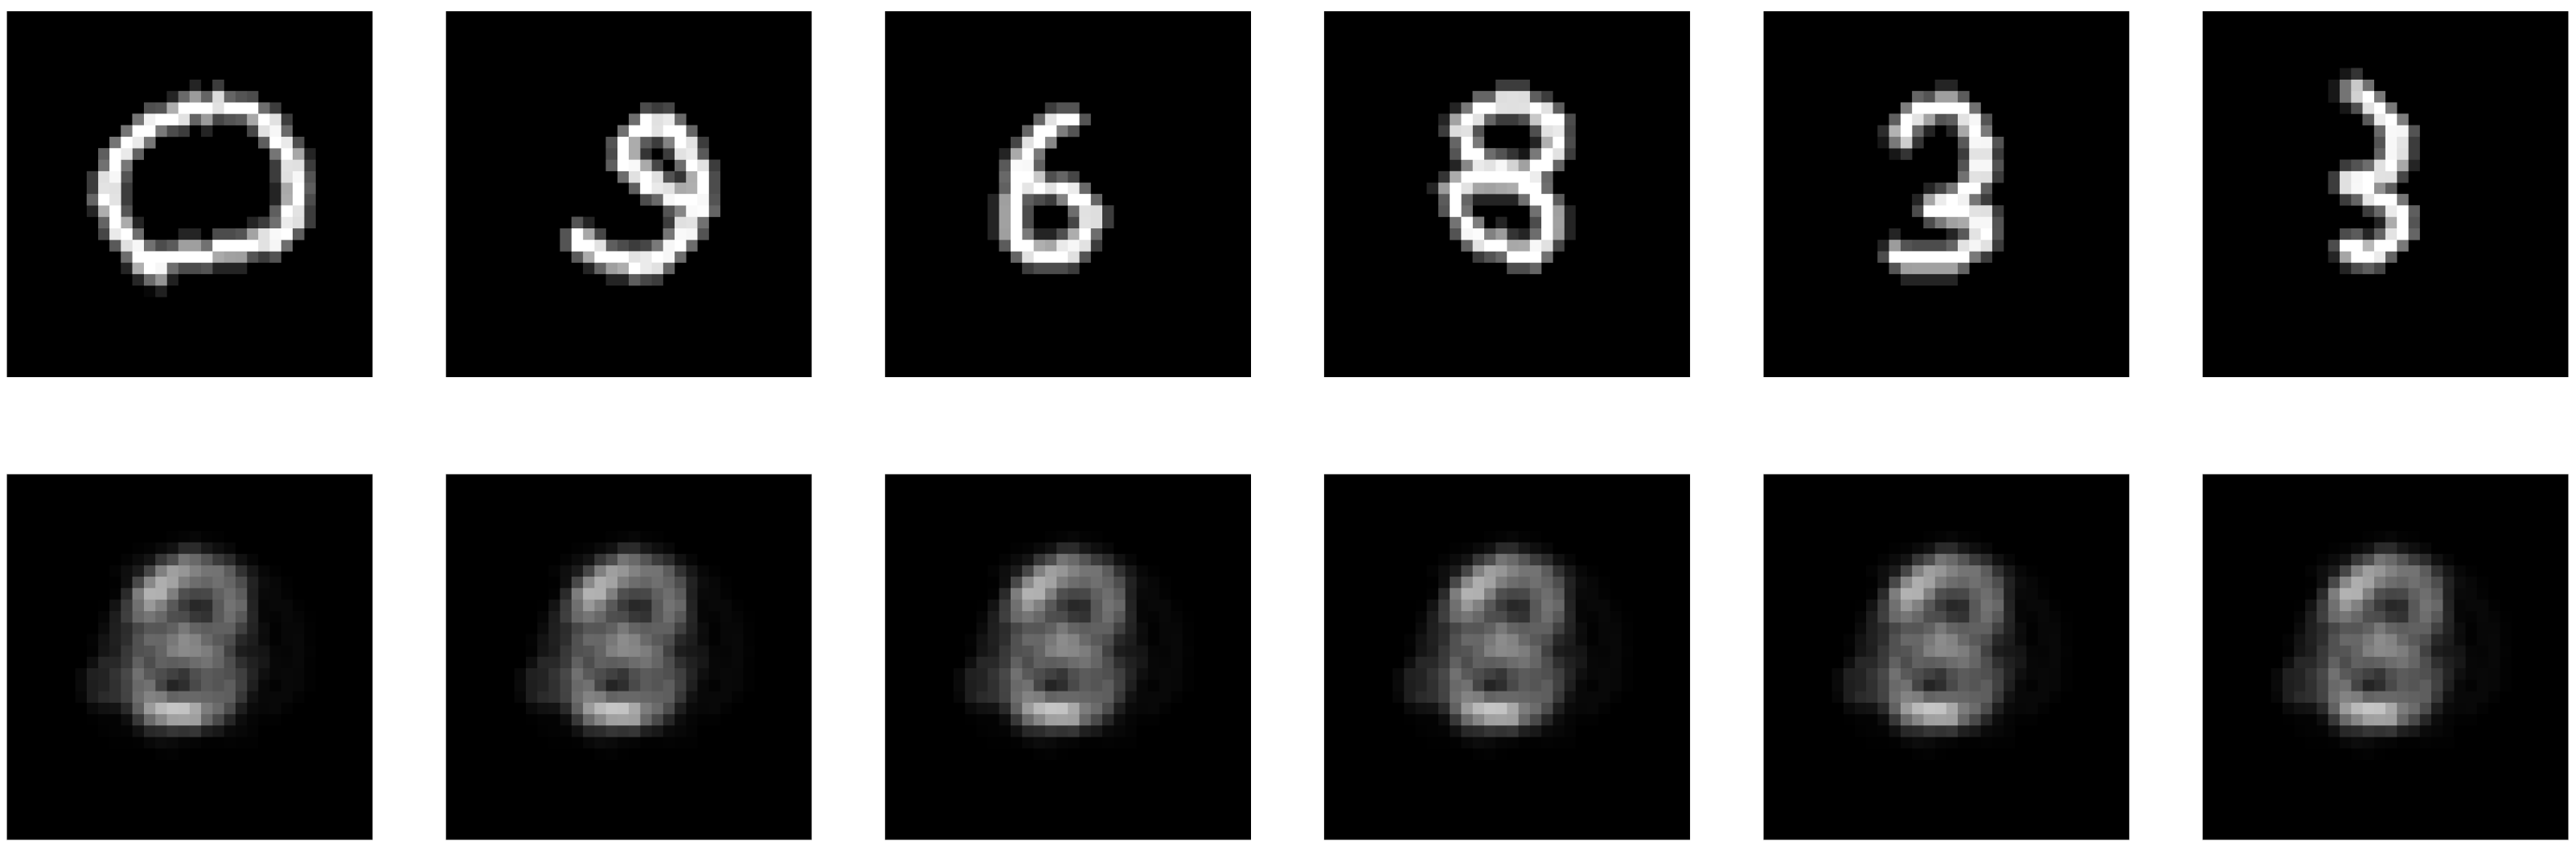
\includegraphics[width=0.7\linewidth]{Figures/FCHopfield1.png}
    \caption{The figure shows how, with a small value of $\beta$, each input gives the same output.}
\end{figure}

\begin{remark}
	$\left\|J_s\right\| = e_1$ where $e_1$ is the largest eigenvalue \\
	Also holds:  \begin{align*}
		\left\|J_s\right\| = e_1 = \text{Tr}\left(J_s\right) - \sum_{i=2}^{n} e_i = \sum_i p_i \text{Tr}\left((x^i-\bar{m})(x^i - \bar{m})^T\right) - \sum_{i=2}^{n} e_i = \sum_i p_i \left\|x^i -\bar{m}\right\|^2 - \sum_{i=2}^{n} e_i
	\end{align*}
	Thus, the bound presented in the previous proposition is high when other eigenvalues are small.
\end{remark}
The previous proposition states that we cannot properly use the Continuous Hopfield Neural Network if the temperature is too high, so it is necessary to formulate some condition for which the network has more than just one attractor point.
\begin{definition}[separation]
	Given a pattern matrix $X$, we define the pattern separation of the $i$-th pattern as:
	\[
	\Delta_i = \min_{j \neq i} (x^i)^Tx^i - (x^i)^T x^j
	\]
	Furthermore, an input $\xi$ is at least separated from $x^i$ while being separated from $x^j$ with $j \neq i$ if:
	\[
	i = \argmax_{k} \min_{j \neq k} (\xi^T x^k - \xi^Tx^j), \quad c =  \min_{j \neq i} (\xi^T x^i - \xi^Tx^j) > 0
	\]
\end{definition}
\begin{lemma}\text{from lemma.A4 in \cite{ramsauer2021hopfieldnetworksneed}}\\
	\label{lemma:Pattern_separation}
	If $\xi$ is at least separated from $x^i$ while being separated from all $x^j$ with $j \neq i$, then:
	\[
	\left\|x^i - f(\xi)\right\| \leq 2 \epsilon M
	\]
	where $M = \max_i \left\|x^i\right\|$ and $\epsilon = (P-1)e^{-\beta c}$
	\begin{proof}
		\begin{align*}
			\left[\softmax(\beta X^T \xi)\right]_i &= \frac{\exp(\beta x^i \xi)}{\sum_j \exp(\beta x^j \xi)} = \frac{1}{1 + \sum_{j\neq i} \exp(\beta \xi^Tx^j-\beta \xi^T x^i)} \geq \frac{1}{1 + \sum_{j\neq i} \exp(-\beta c)} \\
			&= \frac{1}{1 + (P-1) \exp(-\beta c)} = 1 - \frac{ (P-1) \exp(-\beta c)}{1 + (P-1) \exp(-\beta c)} \\
			&= 1 - \frac{\epsilon}{1 + (P-1) \exp(-\beta c)} \geq 1 - \epsilon
			\intertext{given k $\neq i$ then:}
			\left[\softmax(\beta X^T \xi)\right]_k &= \frac{\exp(\beta x^k \xi)}{\sum_j \exp(\beta x^j \xi)} = \frac{\exp(\beta \xi^Tx^k-\beta \xi^T x^i)}{1 + \sum_{j\neq i} \exp(\beta \xi^Tx^j-\beta \xi^T x^i)} \\
			&\leq \frac{\exp(-\beta c)}{1 + \sum_{j\neq i} \exp(\beta \xi^Tx^j-\beta \xi^T x^i)} \leq \exp(-\beta c) = \frac{\epsilon}{P-1}
		\end{align*}
		Now using the definition of $f$, we can prove the proposition:
		\begin{align*}
			\left\|x^i - f(\xi)\right\| &= \left\|x^i - X \softmax(\beta X \xi)\right\| = \left\|(1 - [\softmax(\beta X^T \xi)]_i) x^i - \sum_{k\neq i} x^k [\softmax(\beta X^T \xi)]_k\right\| \\
			&\leq \left(1 - \left[\softmax(\beta X^T \xi)\right]_i\right) \left\|x^i\right\| + \sum_{k\neq i} \left[\softmax(\beta X^T \xi)\right]_k \left\|x^k\right\| \\
			&\leq \epsilon M + \sum_{k\neq i} \frac{\epsilon}{P-1} M  = 2\epsilon M
		\end{align*}
	\end{proof}
\end{lemma}
The previous lemma suggests that separate patterns and $\beta$ not too small will make the sequence defined by the model closer to a particular pattern.
\begin{definition}
	\label{def:Si}
	Given a pattern matrix $X$ we define:
	\[
	S_i = \left\{ \xi \middle| \left\|\xi - x^i\right\| \leq \frac{1}{\beta P M}  \right\}
	\]
\end{definition}
\begin{proposition}\text{from lemma.A5 in \cite{ramsauer2021hopfieldnetworksneed}}\\
	\label{prop:local_conv}
	If $\xi \in S_i$ and $\Delta_i \geq \frac{2}{\beta P} + \frac{1}{\beta} \log(2(P-1)P \beta M^2)$ then: $f(\xi) \in S_i$
	\begin{proof}
		We define $\widetilde{\Delta_i}= \min_{j\neq i} \xi^Tx^i - \xi^T x^j$\\
		Using the  Cauchy-Schwartz inequality, we get: $\left|\xi^Tx^j - (x^i)^Tx^j\right| \leq \left\|\xi - x^i\right\|\, \left\|x^j\right\| \leq \left\|\xi - x^i\right\| M$

		\noindent So we can say that:
		\begin{align*}
			\widetilde{\Delta_i} &= \min_{j\neq i} \xi^Tx^i - \xi^T x^j =  \min_{j\neq i} \xi^Tx^i -\left(x^i\right)^Tx^i + \left(x^i\right)^Tx^i  -\xi^Tx^j + \left(x^i\right)^Tx^j - \left(x^i\right)^Tx^j \\
			&\geq \min_{j\neq i} \left(\left(x^i\right)^Tx^i - \left\|\xi - x^i\right\| M\right) - \left(\left(x^i\right)^Tx^j +\left\|\xi - x^i\right\| M\right) \\
			&= -2\left\|\xi -x^i\right\|M +  \min_{j\neq i} \left(x^i\right)^Tx^i - \left(x^i\right)^Tx^j = \Delta_i - 2\left\|\xi -x^i\right\|M  \\
			& \geq \Delta_i - \frac{2}{\beta P}
		\end{align*}
		Where the last inequality holds because  $\xi \in S_i$.\\
		From \cref{lemma:Pattern_separation} we can affirm that:
		\begin{align*}
			\|x^i - f(\xi)\| &\leq 2 \epsilon M = 2 M (P-1) \exp\left(-\beta \widetilde{\Delta_i}\right) \leq  2 M (P-1) \exp\left(-\beta \left(\Delta_i - \frac{2}{\beta P}\right)\right) \\
			&\leq 2 M \left(P-1\right) \exp\left(-\beta \left( \frac{2}{\beta P} + \frac{1}{\beta} \log\left(2\left(P-1\right)P \beta M^2\right) - \frac{2}{\beta P}\right)\right)\\
			&=  2 M \left(P-1\right) \frac{1}{2\left(P-1\right)P \beta M^2} = \frac{1}{\beta P  M}
		\end{align*}
	\end{proof}
\end{proposition}
Using the previous proposition and \cref{th:statonary_points} we can state that if the input is inside a sphere $S_i$, then the accumulation points, which are points of minima for the energy, are inside the sphere, which allows us to use the network properly, with the right choice of temperature, because different input gives different output.
\begin{remark}
	We can always find a value for $\beta$ that satisfies the condition of the previous proposition $\forall i$  solving:
	\[
	\min_i \Delta_i \geq \frac{2}{\beta P} + \frac{1}{\beta} \log(2(P-1)P \beta M^2)
	\]
	which is equivalent to solving:
	\[
	\beta \geq \frac{2}{P \min_i \Delta_i }+\frac{\log(2(P-1)P M^2)}{\min_i \Delta_i} +\frac{ \log(\beta)}{ \min_i \Delta_i}
	\]
	which solution is: $\beta \in (0,\beta_-] \cup [\beta_+,\infty)$ where $\beta_-,\beta_+$ are the point of \\intersection of $y=x$ and $y=\frac{2}{P \min_i \Delta_i }+\frac{\log(2(P-1)P M^2)}{\min_i \Delta_i} +\frac{ \log(x)}{ \min_i \Delta_i}$. \\
	For retrieval, the smallest solutions are useless because they correspond to the global convergence state of the network, as proved in \cref{prop:J_norm}. However, the largest ones are useful because they can give disjoint $S_i$.
\end{remark}

\begin{figure}[ht]
    \centering
    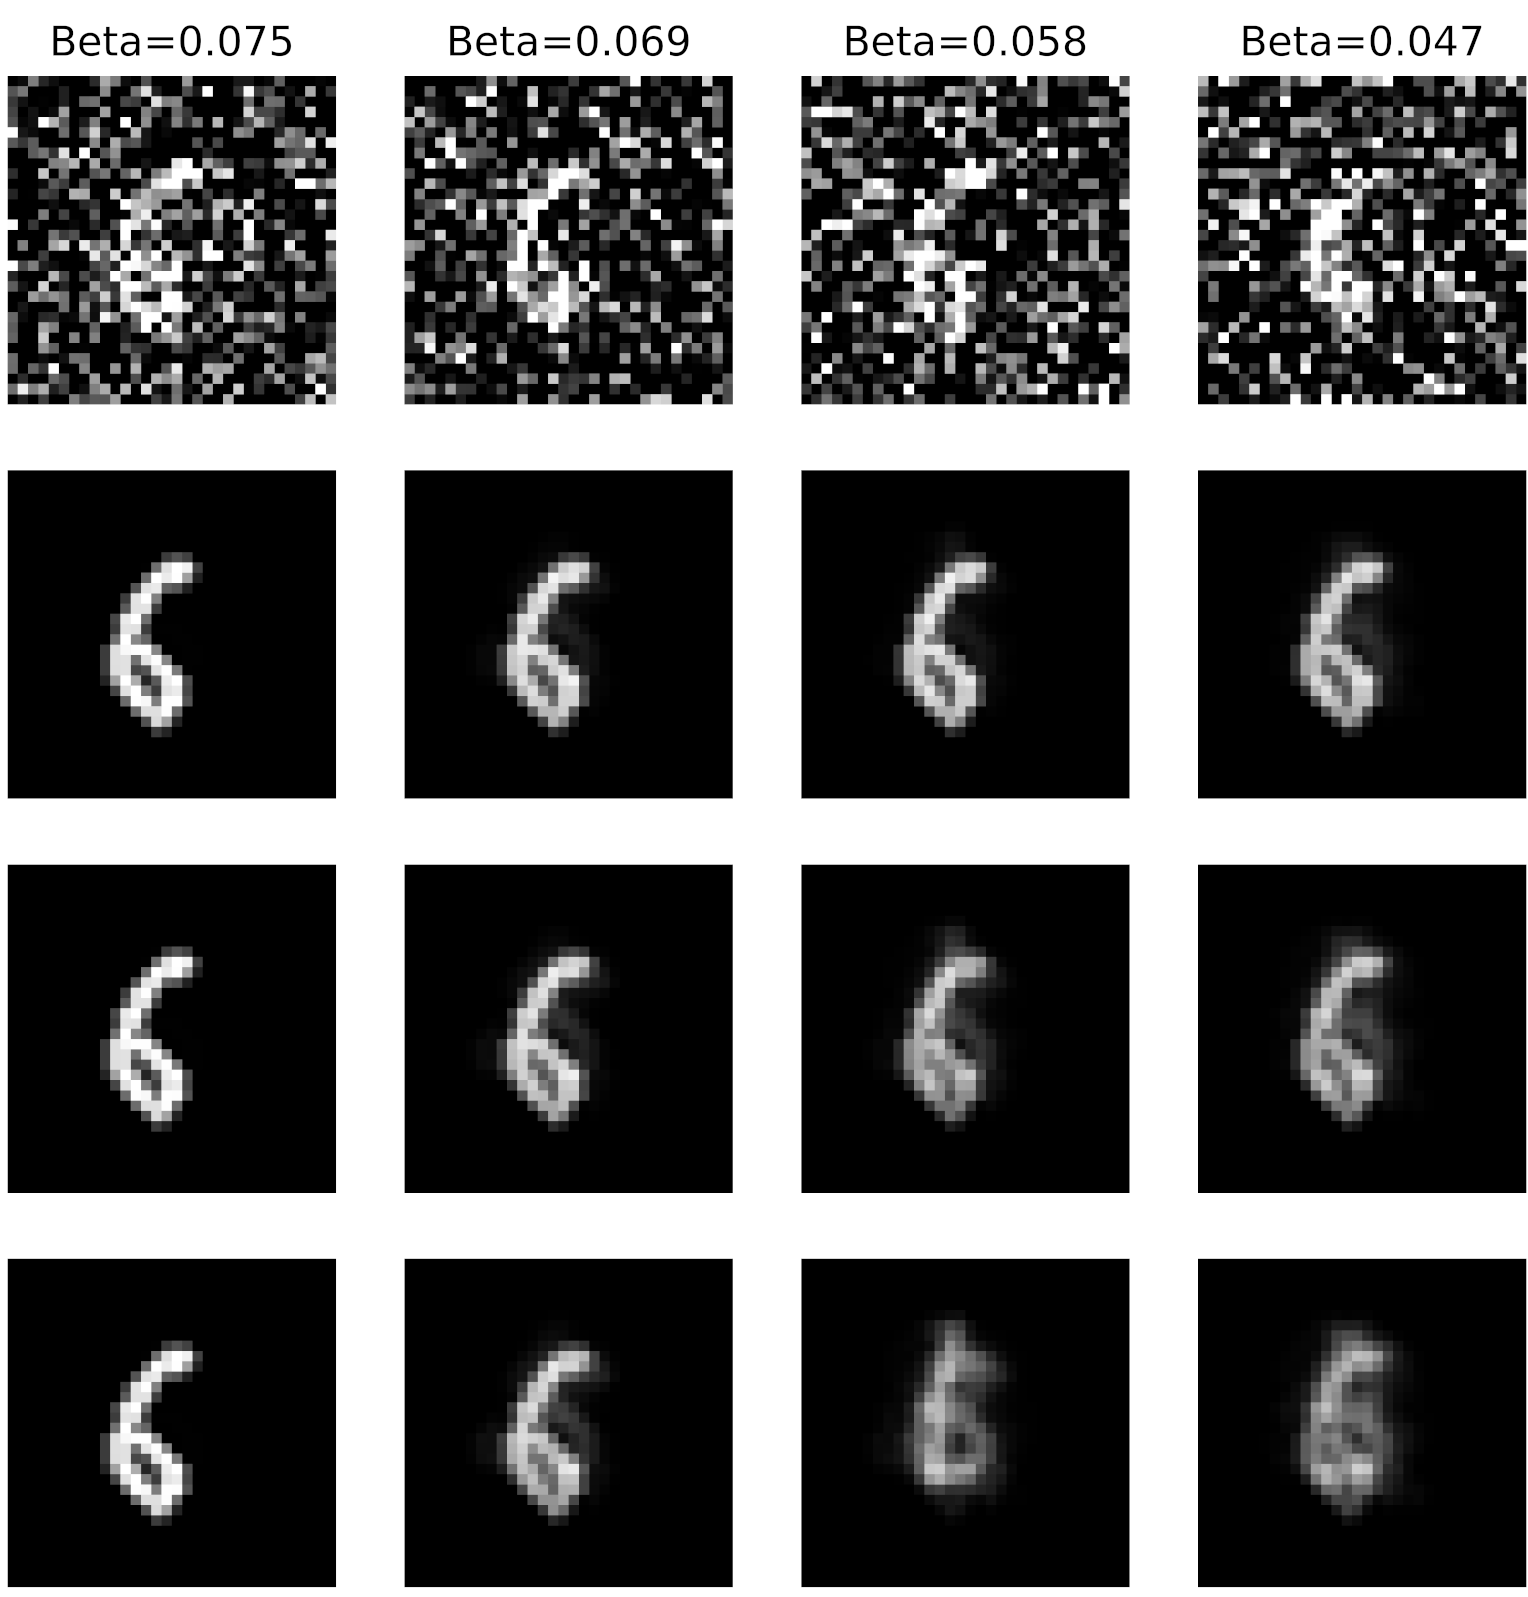
\includegraphics[width=0.6\linewidth]{Figures/FCHopfield.png}
    \caption{The figure shows how the same network gives different outputs with different $T$, larger values bring to a convergence point that is a mixed pattern instead smaller values give local convergence to the stored pattern. The input image is obtained as a random perturbation of a stored pattern.}
\end{figure}

\section{Comparison with discrete Hopfield network}
In this section we want to analyse the differences and analogies between the discrete and the continuum Hopfield networks.
\begin{itemize}
	\item \textbf{Network structure}\\
	Both networks receive an input image, represented as an array of numbers, and process it by correlation with stored patterns. By iteratively updating the input, each network aims to transform it into something closer to a stored pattern.
	\item \textbf{Energy minimization}\\
	An energy function can be defined for both networks, expressed in terms of correlations with stored patterns. This function decreases along the network dynamics and guides the system towards energy minima.
	\item \textbf{Stochasticity and temperature} \\
	Both networks have a parameter called temperature, which can be tuned to facilitate convergence. However, this parameter affects each network differently: in discrete networks, temperature controls the amount of random noise in the updating rule, introducing a degree of stochasticity. In continuous networks, the temperature affects how information is integrated within the softmax operation, so there is no randomness. Despite this difference, the two networks show similar behavior with respect to temperature. In both cases, high temperatures lead to uninformative outputs, where each input is transformed into a generic, uninformative result. Conversely, too low a temperature can also be problematic, leading to trivial outputs in both networks.
	\item \textbf{Pattern and training}\\
	In both networks, the energy function and update rules are defined in terms of stored patterns. However, due to the discrete nature of the neurons, the dynamics of discrete networks cannot be distinguished from the pattern vectors. In contrast, continuous networks allow the computation of derivatives, which allows them to be integrated into larger deep neural networks and trained with backpropagation. Discrete networks, on the other hand, lack any form of learning because the patterns are fixed and remain unchanged.
\end{itemize}

    \chapter{Applications}
\label{ch:Applications}
In this chapter, we will introduce basic implementations and applications of Continuous Hopfield Neural Networks. The results of the contents of this chapter are replicable using the open source repository \cite{github_repo}. We recall contents, techniques and interpretations of the course notes of Deep Learning and Applied Artificial Intelligence of \citet{DLAI}.

\section{Implementations}
In \cref{def:updating}, we defined the updated state of a Hopfield neural network as:
\[
\xi^{\text{new}} = X \softmax \left(\beta X^T \xi\right)
\]
This neural network is used to classify inputs, so it is more informative to study the evolution of the logits. A \textbf{logit} represents the degree to which an input adheres to a particular feature. For example, the image of a '$1$' may resemble that of a '$7$', meaning that the '$1$' may have a high logit for feature '$7$'. Typically, the softmax of all logits represents the probability that the $1$ is classified as a $7$ in this case. Note that the vector of logits is proportional to the vector of magnetisations for each pattern, in particular $l_\mu = N\beta m_{N,\mu}(\xi)$ from \cref{def:mattis_mgn}.

\noindent An equivalent way to express the update formula using logits is
\[
l^{\text{new}} = \beta X^T \xi^{\text{new}} = \beta X^T X \softmax \left(l\right)
\]
We define $A_\beta \mathdef \beta X^T X$, so $l^{\text{new}} = A_\beta \softmax \left(l\right)$. A Hopfield neural network can be thought of as a cyclic \texttt{FCL} with softmax activation:

\begin{figure}[htbp]
	\centering
	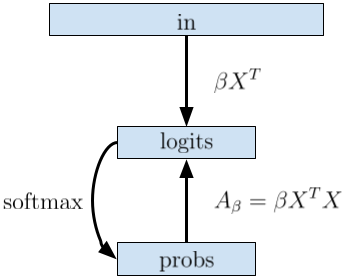
\includegraphics[width=0.4\linewidth]{Figures/FCL.png}
	\caption{Diagram of the Hopfield neural network. The input (on the top) passes through a fully connected layer with parameters $\beta X^T$ and zero bias. The logits are then fed into a cyclic loop, and the output is obtained. To reconstruct the image, we can use the \textit{probs} layer; $Xp=\xi$, so we can connect an FC layer without bias and weights $X$ to the \textit{probs} layer.}
	\label{fig:FCL}
\end{figure}

\paragraph{Convolutions} A Hopfield neural network looks at the whole image and analyses the image as a whole. To restrict the analysis to a smaller Hopfield neural network, we can define a convolution of the Hopfield neural network. This allows us to reconstruct small patterns in more small parts of the image. A convolution returns a new image with more (or less) channels with logits, and each logit indicates the presence of a pattern in the image.

\noindent Let $H$ be a Hopfield neural network that takes $C_i \times S$ neurons as input and returns $C_o$ logits, where $S$ is a shape (e.g. $3 \times 3$) with $n$ dimensions. A convolution applies $H$ to each region of shape $S$ in data with $C_i$ channels and $n$ dimensions.

\noindent For example, if we have an image of size $32 \times 32$ with $3$ channels (\texttt{RGB}), we can apply a convolution with a $4 \times 4$ filter. In this case $H$ operates on $3 \times 4 \times 4 = 48$ neurons and detects $5$ patterns. The convolution returns data with $5$ channels and a shape of $29 \times 29$, where each position represents the response to a pattern for that region of the image.

\noindent In \cref{fig:CNN} we can see that a convolution works in a similar way to a classical Hopfield neural network.
\begin{figure}[htbp]
    \centering
    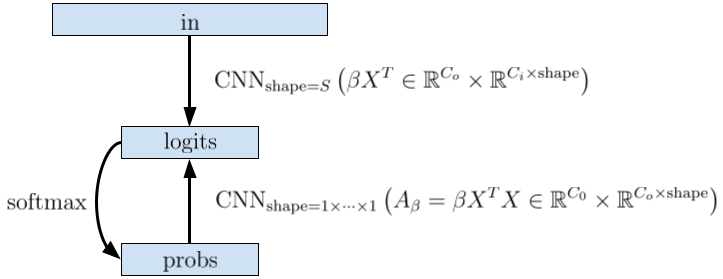
\includegraphics[width=0.8\linewidth]{Figures/CNN.png}
    \caption{The neural network receives data in the form of $C_i \times S$. A convolutional layer computes the logit vector for each region, producing data in the form of $C_o \times S$. A pointwise softmax is then applied to each logit vector. Finally, each logit vector is linearly transformed and a pointwise convolutional layer is applied, producing data of the form $C_o \times S$.}
    \label{fig:CNN}
\end{figure}

\begin{remark}[Generalized Continuous Hopfield Neural Networks]
	During training, the parameters of a Hopfield neural network can become difficult to interpret. Is it possible to train a number of parameters that is not directly proportional to the number of neurons?

	\noindent The matrix $A_\beta$ is not arbitrary. In fact, it must satisfy the following properties:
	\begin{itemize}[itemsep=2pt, topsep=10pt]
		\item $A_\beta$ is a real, square, and symmetric matrix.
		\item $A_\beta$ is non-negative: $v^T A_\beta v = \beta v^T X^T X v = \beta \|Xv\|^2 \geq 0$.
	\end{itemize}
	Therefore, if interpretability is not an issue, we can train over a matrix $M \in \mathbb{R}^{C \times C}$ and set $A_\beta = M^T M$. In this way the Hopfield neural network can be seen as a composition of: a \texttt{FC} layer with parameter $\beta X^T$ and bias $0$, a cycle with $A_\beta = M^T M$, and another \texttt{FC} layer with parameter $X$ and bias $0$.

	\noindent This observation also applies to convolutional Hopfield nets.
\end{remark}

\paragraph{Autoencoders}
Note that the number of parameters $P$ is much smaller than the number of neurons $N$, so image reconstruction using Hopfield neural networks is a special case of \textbf{autoencoder}. In fact, the Hopfield neural network reduces the dimensionality of the input (with $N$ neurons), then it recalls the pattern in the loop and reconstructs the image from it, in detail:
\[
XH_{\beta,X}\left(\xi\right) = XH_{A_\beta}'\left(\beta X^T\xi\right)
\]
where $H$ is the main Hopfield neural network with $N$ neurons and $P$ patterns, $H'$ is a Hopfield neural network with $P$ neurons and $P$ patterns. $\beta X^T$ makes the code of $\xi$ (encoding), this code is cleaned in the loop (in a manifold) and finally it is rebuilt (decoding).

\noindent Now we derive a variational autoencoder from Hopfield neural networks and \textit{PCA}. We observe that a Hopfield neural network is a variant of a \textit{PCA} because it uses a matrix and its transpose to encode and decode information, the only difference being an additional softmax layer, an internal loop, and an initial and final multiplicative constant\footnote{For more about PCA, see \url{https://www.cs.umd.edu/class/spring2019/cmsc422-0101/materials/lecture20-sp19.pdf}}. So we get a \textit{PCA} similar to a Hopfield net:
\begin{itemize}
    \item \textbf{encoding} : The input is multiplied by $\sqrt{\beta}X^T$.
    \item \textbf{decoding} : The code is multiplied by $\sqrt{\beta}X$.
\end{itemize}
Now we turn this autoencoder into a variational autoencoder. So the encoder returns information about some probability distribution and the decoder samples from that distribution and reconstructs the input, this is a \textbf{VAE}\footnote{For more about VAEs, see \url{https://www.ibm.com/think/topics/variational-autoencoder}}. We can see that a Hopfield neural network has the same architecture, but it has no sampling. The final architecture is shown in \cref{fig:VAE}.
\begin{figure}[htbp]
    \centering
    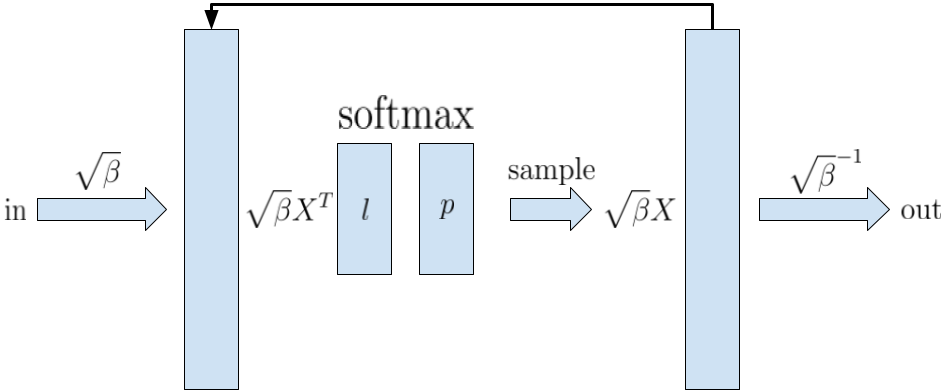
\includegraphics[width=0.9\linewidth]{Figures/VAE.png}
    \caption{The input is passed to the autoencoder with a simple multiplication ($\sqrt{\beta}$), then the autoencoder multiplies its input by $M^T$, this produces a vector of $P$ logits $l$, after a softmax we get a discrete distribution $p$. Now it's possible to simulate this distribution with one or more samples. This distribution is then passed to the decoder which multiplies it by $M$. This is a single loop and we can answer it using the output as a new input.}
    \label{fig:VAE}
\end{figure}

\section{DeepHNN}
First, we define a simple use of Hopfield neural networks. A \textbf{DeepHNN} is a Hopfield neural network with more patterns given the number of target features. In fact, using $3$ patterns per feature may be better than using only one pattern per feature. Thus, the logit returned by a DeepHNN is the maximum logit for any subset of patterns returned by a Hopfield neural network.

\begin{figure}[ht]
    \centering
    \begin{minipage}{0.45\textwidth}
        \centering
        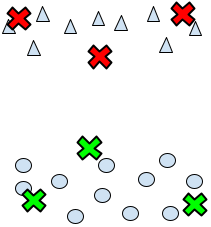
\includegraphics[width=0.6\linewidth]{Figures/DeepHNN.png}
    \end{minipage}
    \hfill % Spazio orizzontale tra le figure
    \begin{minipage}{0.45\textwidth}
        \centering
        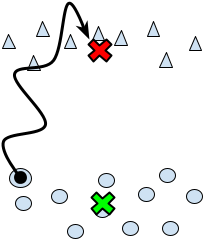
\includegraphics[width=0.6\linewidth]{Figures/DeepHNN_1.png}
    \end{minipage}
    \caption{We have two features: triangles and circles. By using $3$ patterns per feature, we can better capture the data with better coverage. However, the result may be more confusing.}
    \label{fig:DeepHNNDiagram}
\end{figure}

\noindent We have added a \textbf{final bias} for each pattern in the same feature. The bias can assign a confidence about a feature, it is very useful to interface with other layers. In a classical Hopfield neural network the bias is the same for each feature, but when there are other layers and in a more complex neural network it is better to add a new degree of freedom. In algorithm \ref{alg:HNN_forward} we show an excerpt of the code used for the forward pass. In particular, the implemented class \texttt{DeepHNN} uses more channels, a separate neural network for each channel.

\newpage

\begin{lstlisting}[style=code, label=alg:HNN_forward, caption=DeepHNN forward pass, language=Python]
import torch
from torch import nn
from torch.nn import functional

""" method of DeepHNN
attributes:
    iterations: int
    channels, features, deep, neurons: int
        positive values
    _logbeta: nn.Parameter
        with shape (channels,)
    _bias: nn.Parameter
        with shape (channels, features,)
    _patterns: nn.Parameter
        with shape (channels, deep * features, neurons,)
"""
def forward(self, x: torch.Tensor) -> torch.Tensor:

    # Shape of x must be (batch, channels, neurons)

    L = torch.exp(self._logbeta).view(self.channels, 1, 1) * self._patterns
    A = torch.einsum('cin , cjn-> cij', L, self._patterns)  # i,j are logits

    # main algorithm
    x = torch.einsum('cln, bcn -> bcl', L, x)  # get logits
    for _ in range(self.iterations):
        x = functional.softmax(x, dim=2)  # get probs
        x = torch.einsum('clp, bcp -> bcl', A, x)  # get logits

    # max reduction
    x = x.view(-1, self.channels, self.features, self.deep)
    x = torch.max(x, dim=3).values
    x = x + self._bias.view(1, self.channels, self.features)

    return x
\end{lstlisting}

\paragraph{A Simple Experiment}
The first experiment applies a Hopfield neural network with predefined patterns directly to an MNIST image. We manually define $3$ patterns for each digit between $0$ and $9$, and then implement a Hopfield neural network over $32 \times 32$ neurons. In \cref{fig:SimpleExp} we observe that the neural network has trouble recognizing the true digit. To solve this problem, we can try to train the neural network on MNIST and then analyze the results.

\begin{figure}[htbp]
    \centering
    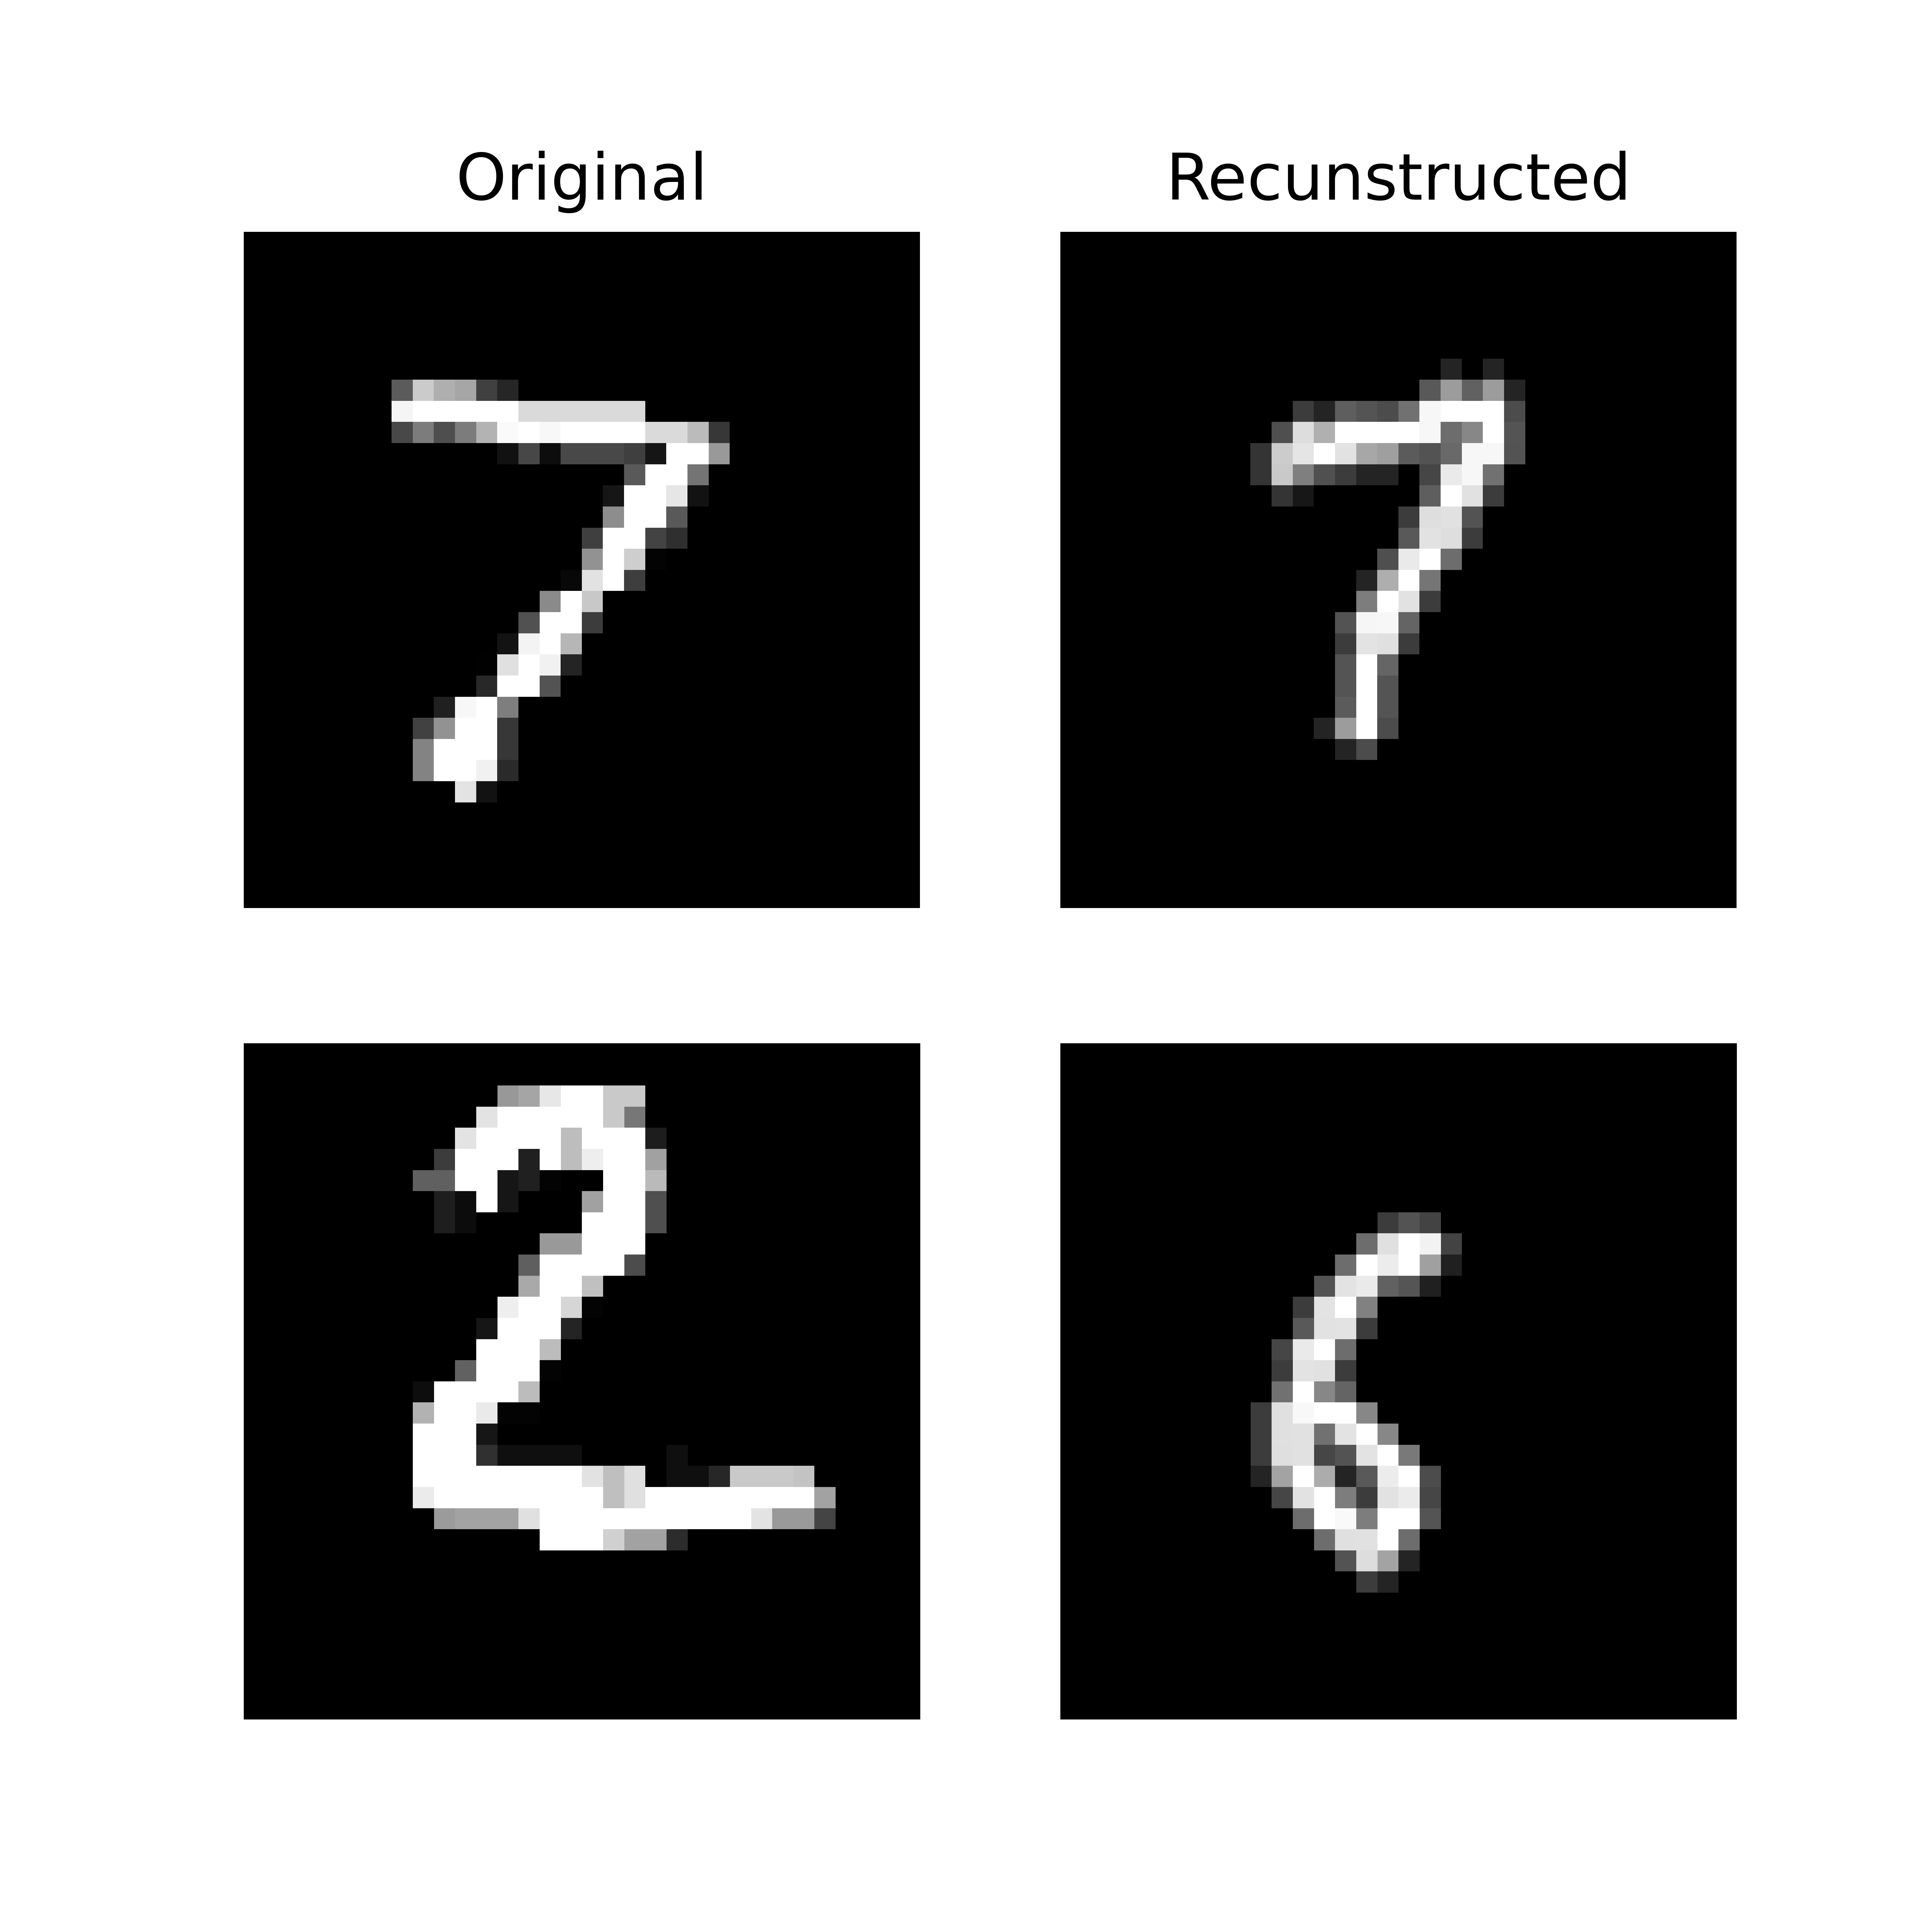
\includegraphics[width=0.5\linewidth]{Figures/SimpleExp.png}
    \caption{Applying a Hopfield neural network to two MNIST images. The Hopfield neural network had $\beta = 0.07$ and ran for 2 iterations.}
    \label{fig:SimpleExp}
\end{figure}

\noindent The neural network was trained using the cross-entropy loss for $40$ epochs with an adaptive learning rate using the current accuracy. At the end of training, the cross-entropy loss was $1.8$, and in the test phase, the neural network showed $32\%$ accuracy. The patterns with high attribution influence were not changed.

\paragraph{DeepHNN as MLP}
A single Hopfield neural network with the whole image as input is often not the best choice, because the output of the neural network depends entirely on the dot product with the vector patterns, i.e. moving all the pixels to the right (or left, or up, or down) will give a completely different output. Furthermore, we can observe that within a Hopfield neural network there is no notion of locality, in fact patterns are retrieved if and only if they are in the same position of the stored patterns. To overcome these problems, we observe that more smaller neural networks are better than only one, because they can analyze a small part of the images.

\noindent A convolution can create more "versions" of the same image, in particular it highlights a set of patterns in the image. For example, a convolution that detects horizontal lines and vertical lines will show, with high values, where there are horizontal lines and vertical lines. Thus, a single-channel image becomes a multichannel image (one for each feature). In addition, the number of patterns is usually not too large in relation to the number of input channels and the size of the kernel. Typically, the number of patterns is a quarter of the number of neurons in a kernel (e.g., $8$ input channels, $4\times4$ kernel size, $32$ output channels).

\noindent We define a neural network with a linear CNN that has $5$ channels with $4\times4$ kernels and $2$ steps. Then we use a DeepHNN with $5$ channels and $10$ features with deep $5$. Finally, we add a trainable convex reducer that merges all channels into only one and obtains $10$ logits. This neural network has $\num{56440}$ trainable parameters. We trained this neural network for $40$ epochs with a learning rate of $0.01$: the final accuracy obtained is $\approx87\%$ with a cross entropy loss of $0.7$. In \cref{fig:asMLP} it's possible to see details about the training, but kernels and patterns are not visible.

\begin{figure}[htbp]
    \centering
    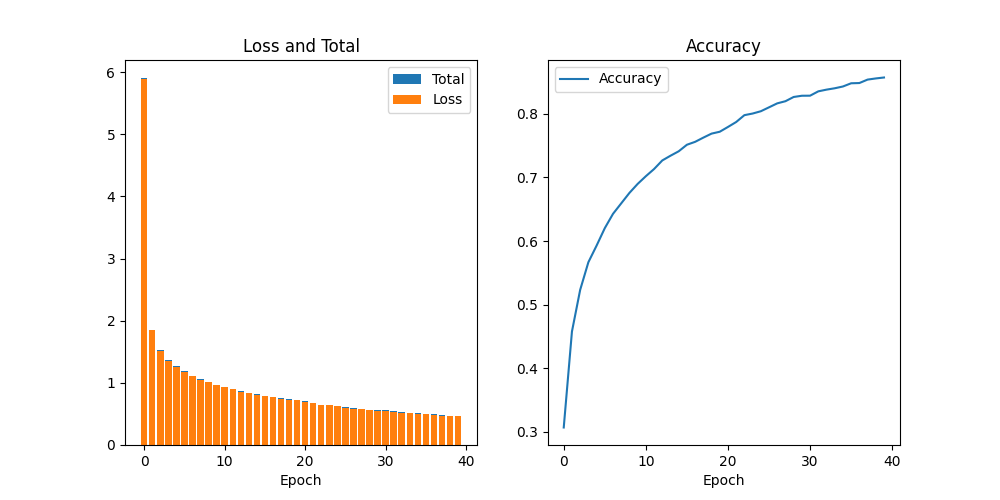
\includegraphics[width=0.9\linewidth]{Figures/asMLP.png}
    \caption{On the left the loss evolution during training (in orange the cross entropy loss, in blue the part due to the regularization), on the right the accuracy evolution.}
    \label{fig:asMLP}
\end{figure}

\section{ConvHNN2d}
We define a convolutional layer with Hopfield as a small Hopfield neural network that detects patterns in all parts of the image (see \cref{fig:CNN}). In this experiment, we use a $2d$ convolution to use over MNIST.

\noindent The main difference between a typical linear convolution and this convolution is how it highlights the patterns. A linear convolution pattern works over logits, so if it looks for the pattern $\left(1,1\right)$, it will highlight the pattern $\left(5,5\right)$ with value $10$ (excellent compatibility) and the pattern $\left(1,1\right)$ with value $2$ (good, but not excellent). So it works not in terms of distance, but in terms of the scalar product (intensities and directions) of patterns. A Hopfield neural network looks at patterns in a different way and does not work in terms of distance or scalar products. The Hopfield neural network tries to recall a pattern so that the final image is a mixture of recalled patterns for each region of the image, so it can clean the image from noise, and this behaviour is very useful when this neural network is the first convolutional layer. In the algorithm \ref{alg:CNN_forward} we show the forward pass of this layer.

\newpage
\begin{lstlisting}[style=code, label=alg:CNN_forward, caption=ConvHNN2d forward pass, language=Python]
import torch
from torch import nn
from torch.nn import functional

""" method of ConvHNN2d
attributes:
    channels_in, channels_out: int
        positive values
    kernel_size, padding, stride, dilation
        parameters of classical convolution
    iterations: int
        number of neurons of theoretical Hopfield neural network
    _logbeta: nn.Parameter
        with shape (1,)
    _bias: nn.Parameter
        with shape (channels_out,)
    _patterns: nn.Parameter
        with shape (channels_out, channels_in, kernel_size)
"""
def forward(self, x: torch.Tensor) -> torch.Tensor:

    # Shape of x must be (batch, channels_in, #, #)

    weight_loop = (
        torch.exp(self._logbeta)
        * torch.einsum(
            'in, jn -> ij',  # i,j are logits (channels_out)
            self._patterns.view(self.channels_out, -1),
            self._patterns.view(self.channels_out, -1)
        )
    ).view(self.channels_out, self.channels_out, 1, 1)

    x = nn.functional.conv2d(
        x,
        torch.exp(self._logbeta) * self._patterns,
        stride=self.stride,
        padding=self.padding,
        dilation=self.dilation,
    )
    for _ in range(self.iterations):
        x = nn.functional.softmax(x, dim=1)
        x = nn.functional.conv2d(x, weight_loop)

    return x + self._bias.view(1,self.channels_out,1,1)
\end{lstlisting}

\noindent In this experiment, we define a simple neural network that attempts to reconstruct an image using only convolutions. In particular, the input image has Gaussian noise, so we will use ConvHNN2d to remove the noise and reconstruct the original image. A Hopfield convolution produces an image with $C_{\text{out}}$ logits per pixel, so for each vector of logits per pixel we can recall the pattern using this formula:
$$
    \text{recalled pattern} = X\softmax\left(\text{logits}\right)
$$
Thus, the transposed convolution combines all the reconstructed patterns and obtains an approximation of the original convolution. In our architecture, a ConvHNN2d uses $9$ patterns with kernel size $(5,5)$. Thus, it produces a new image with $9$ channels of logits, the bias penalizes the patterns related to the noise and rewards the real patterns. In this way, the transposed convolution reconstructs only good patterns.

\begin{figure}[htbp]
    \centering
    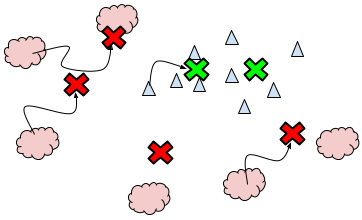
\includegraphics[width=0.6\linewidth]{Figures/anti-noising.png}
    \caption{Patterns with low bias (in red) are ignored as logits. In this way these patterns protect correct patterns with higher bias.}
\end{figure}

\noindent The architecture of the neural network is detailed:
\begin{itemize}
    \item \texttt{ConvHNN2d} with $9$ patterns and $5\times5$ kernel size and a \texttt{SiLU} activation
    \item \texttt{AutoEncoder} with: a linear convolution of $9$ channels to $3$ channels and $3\times3$ kernel size as encoder, a transposed convolution of $9$ channels to $2$ channels and $3\times3$ kernel size as decoder.
    \item Transpose convolution with Hopfield parameters.
\end{itemize}
This neural network was trained to reconstruct images, so its input was an image with Gaussian noise (with variance $1.0$). After training $20$ epochs, the MSE loss over the test set is $4 \times 10^{-2}$ with only $742$ trainable parameters.

\noindent Now we see how this neural network cleans up the images. In \cref{fig:CNNexample} we show the evolution of an image through the neural network.
\begin{figure}[htbp]
    \centering
    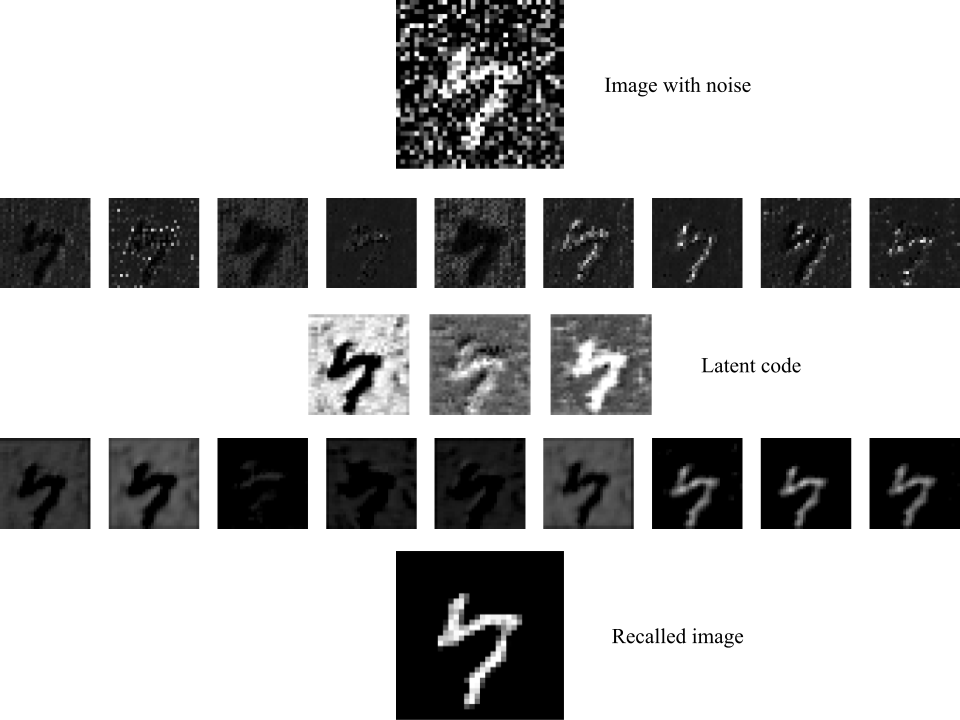
\includegraphics[width=1.0\linewidth]{Figures/CNNexample.png}
    \caption{Above is an image from MNIST with Gaussian noise (variance: $1.44$). The Hopfield convolution layer highlights certain patterns in the image (see white pixels). A linear CNN finds $3$ patterns from logits. An activation function then removes the residual noise so that a transposed CNN reconstructs the logits of the Hopfield convolution. Finally, the patterns from the Hopfield convolution are used to reconstruct the original image without noise.}
    \label{fig:CNNexample}
\end{figure}

\section{Variational Hopfield Neural Network (VHNN)}
In \cref{fig:VAE} we showed the architecture of the Variation Hopfield Neural Network, we observe that the number of samples defines the incidence of noise. If we get a single sample from the distribution $p$ we will have maximum noise, if we get a lot of samples the neural network will look like a typical Hopfield neural network.

\noindent We observe that $p = \mathbb{E}_p\left[M^n\right]$ where $M^n$ is the estimated distribution from $n$ Bernoulli samples from the distribution $p$. Let $M^n_k$ be the $k$th estimate associated with the $k$th sample (or the $k$th component of the softmax operation) and $\sigma_k$ be the variance of the Bernoulli sample from the $k$th component.
\[
\frac{M_k^n - p_k}{\sigma_k / \sqrt{n}} = \frac{\frac{1}{n}\sum^n \text{Be}(p_k) - p_k}{\sigma_k / \sqrt{n}} \overset{D}{\to} \mathcal{N}\left(0,1\right)\,,\quad \quad \sigma^2 = \text{Var}\left[\text{Be}(p_k)\right] = p_k(1-p_k)
\]
We can reformulate the noise with an approximation:
\[
S^\eta \mathdef p + \text{diag}\left(\sqrt{p_k(1-p_k)}\right)\varepsilon\,, \quad \quad \varepsilon \sim \mathcal{N}\left(0,\eta^2\mathds{1}\right)\,,\quad \eta\in\mathbb{R}_+
\]
where $S^\eta$ is the sampled data from the distribution $p$ in \textbf{VHNN}. Note that the noise $\eta$ is a continuous and eventually trainable value that replaces the iper parameter $\frac{1}{\sqrt{n}}$.

\noindent This formulation is very similar to the common formulation of VAE, which uses normal samples from the mean and variance given by the encoder.

\noindent In algorithm \ref{alg:VHNN_forward} we show the forward pass of layer VHNN.

\begin{lstlisting}[style=code, label=alg:VHNN_forward, caption=VHNN forward pass, language=Python]
import torch
from torch import nn
from torch.nn import functional

""" method of ConvHNN2d
attributes:
    channels, features, neurons: int
        positive values
    iterations: int
        number of neurons of theoretical Hopfield neural network
    _logbeta, _lognoise: nn.Parameter
        with shape (channels,)
    _patterns: nn.Parameter
        with shape (channels, features, neurons)
"""
def forward(self, x: torch.Tensor) -> torch.Tensor:

    # Shape of x must be (batch, channels, neurons)

    L = torch.exp(self._logbeta/2).view(-1, 1, 1) * self._patterns

    x = torch.exp(self._logbeta/2).view(1, -1, 1) * x
    for _ in range(self.iterations):
        x = torch.einsum('cfn, bcn -> bcf', L, x)
        x = nn.functional.softmax(x, dim=2)
        epsilon = torch.randn_like(x, device=x.device, requires_grad=False)
        xdet = x.detach().requires_grad(False)
        x = x + torch.exp(self._lognoise).view(1,-1,1) * (xdet*(1-xdet))**0.5 * epsilon
        x = torch.einsum('cfn, bcf -> bcn', L, x)

    x = torch.exp(-self._logbeta/2).view(1, -1, 1) * x
    return x
\end{lstlisting}

\paragraph{A Simple Experiment}
Using the noise, we study how the state evolution falls into and escapes from a $S_i$ (see \cref{prop:local_conv}).

\noindent Now we analyze the pattern set $S$ with $30$ patterns in the previously used $\mathbb{R}^{32\times32}$. We calculate the values $M$ and $\left(\Delta_i\right)_i$:
\[
M=\max_\mu \|x^\mu\| = 31.3933
\]
\[
\left(\Delta_i\right)_i=\left(\min_{j\neq i} (x^i)^Tx^i - (x^i)^Tx_j\right)_i = \text{ see \cref{tab:Delta}}
\]
\begin{table}[ht]
    \centering
    \begin{tabular}{|>{\columncolor{mint}}c||c|c|c|}
        \hline
        \rowcolor{lavender}
        digit     & pattern $1$ & pattern $2$ & pattern $3$ \\
        \hline
        $0$ & $88.0986$ & $80.1672$ & $131.736$ \\
        \hline
        $1$ & $53.4877$ & $69.0222$ & $59.4534$ \\
        \hline
        $2$ & $63.2126$ & $63.9695$ & $69.7267$ \\
        \hline
        $3$ & $65.0894$ & $55.4366$ & $46.0532$ \\
        \hline
        $4$ & $66.9539$ & $62.2354$ & $46.1037$ \\
        \hline
        $5$ & $41.8603$ & $39.9262$ & $37.5255$ \\
        \hline
        $6$ & $45.8450$ & $60.8577$ & $49.2501$ \\
        \hline
        $7$ & $55.7401$ & $51.3837$ & $35.1906$ \\
        \hline
        $8$ & $52.2477$ & $56.2899$ & $69.4982$ \\
        \hline
        $9$ & $107.129$ & $74.5176$ & $51.1973$ \\
        \hline
    \end{tabular}
    \caption{}
    \label{tab:Delta}
\end{table}

\noindent So we want to find a value $\beta$ such that
\[
    \forall i\left(\Delta_i\geq\frac{2}{\beta P} + \frac{1}{\beta}\log\left(2\left(P-1\right)P\beta M^2\right)\right)
\]
We calculate the minimum value $\Delta_{\min} = \min_i \Delta_i = 37.5255$ and simplify the equation:
\[
    \beta' \geq a + \log\beta'
\]
where: $\beta'=\beta\Delta_{\min}$, $a=\frac{2}{N}+\log\frac{2(N-1)NM^2}{\Delta_{\min}}$

\noindent If $a\leq1$ then the statement holds for any $\beta'$, otherwise we solve the equation $\beta'=a+\log\beta'$. The equation has solutions $\beta'_- < 1$ and $\beta'_+>1$.
We can use a fixed point iteration to find $\beta'_+$ with starting point $u_0=2a$ and $K$ iterations, so we know that $\beta = \frac{u_K}{\Delta_{\min}}$ is a good value for $\beta$, but we could choose a larger one. Now we can calculate the radius of each $S_i$: $R(S_i) \mathdef \frac{1}{\beta N M}$.

\noindent So we calculate $\beta = 0.0727$, but in this experiment we use $\beta=0.063$, which reduces the ability of the neural network to detect patterns. We set the noise to $\beta=0.3$ (high noise) so that we can see a change in opinion very quickly. The VHNN works over $4$ different states: for two patterns the noise does not allow an easy exit from local convergence, while for two patterns the neural network state jumps from one to the other. Empirically, with random inputs we have only these solutions, even if we start from a different $S_i$.

\noindent This is a stochastic process where the state of the neural network is a continuous distribution in the affine space of the patterns. In this way, the neural network can recall other patterns in a manner similar to a classical Markov chain. In a training process, the neural network can choose the position of the patterns to create a particular distribution, and the noise can take values that allow for fast training.

\begin{figure}[htbp]
    \centering
    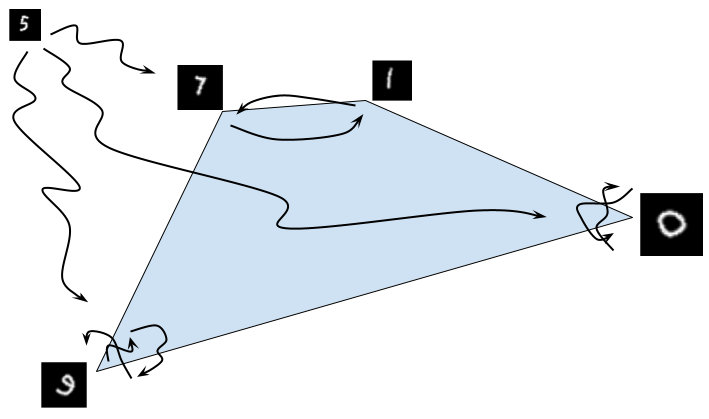
\includegraphics[width=0.6\linewidth]{Figures/VHNNdiagram.png}
    \label{fig:VHNNexample}
\end{figure}

    \chapter{Conclusion}

% recap generale
Although discrete Hopfield networks are a fundamental model in the field of neural networks, they have structural limitations that limit their applicability in modern deep learning architectures. However, their ability to store and retrieve even partially damaged patterns makes them useful in contexts such as pattern recognition and error correction, especially in resource-constrained environments. Acting as "associative memories", they store and retrieve patterns in the presence of partial or noisy inputs, making them particularly effective in areas such as image recognition or error correction in telecommunications. Their rapid stabilization toward an equilibrium state also makes them useful in models of biological behavior. However, their limited memory capacity and inability to be trained by backpropagation reduce their effectiveness in more complex applications.

\noindent Despite their advantages, discrete Hopfield networks suffer from significant limitations in their storage capacity and lack of trainability via backpropagation methods, making them unsuitable for more complex applications. Pattern storage is limited by the fact that the maximum number of patterns that can be stored increases linearly with the number of neurons, making the model ineffective on a large scale. In addition, the lack of gradient descent trainability prevents optimization for more sophisticated applications. These limitations have led to the development of continuous Hopfield networks, which offer greater flexibility, better generalization, and a wide range of applications, especially when integrated with other neural layers.

% Applicazioni e risultati
\noindent To overcome the limitations of discrete networks, continuous Hopfield networks have proven to be a powerful tool, especially when integrated with layers that exploit their properties. In our analysis, we have experimented with several structures that apply the principles of continuous networks to achieve remarkable results. The \texttt{DeepHNN} layer allows multiple patterns to be associated with a single feature, improving the robustness of information retrieval, while \texttt{ConvHNN} overcomes the problem of pattern translation through local analysis, which is more effective than traditional convolutions at removing noise. The \texttt{VHNN model}, which combines continuous Hopfield networks and variational autoencoders (VAE), allows more efficient training and provides theoretical insights into the search for energy minima in stochastic processes. Although continuous Hopfield networks are simpler than other neural architectures, their small number of parameters makes them ideal for resource-constrained environments. In addition, their clustering capability makes them more resistant to overfitting, which improves generalization. However, the training speed is slower than for more complex models and requires optimizers with high learning rates and moderate batch sizes for good convergence, with computational cost increasing with the number of iterations.

% Conclusioni e sviluppi futuri
\noindent A possible future development concerns the theoretical analysis of the behavior of variational Hopfield networks (VHNNs), which raises numerous theoretical questions, such as Is there a limit distribution for stochastic processes in Hopfield networks? What is the waiting time before the network changes state, and how is it related to the energy associated with a state? How do Hopfield networks behave as the number of neurons (or pixels) tends to infinity? Answering these questions could lead to significant theoretical developments in the field of complex dynamical systems and stochastic neural networks, improve the training efficiency of Hopfield networks, and open new avenues for applications in systems theory, optimization, and theoretical machine learning.


\backmatter

    \bibliography{bibliography}

    \phantomsection
    \addcontentsline{toc}{chapter}{\bibname}

\end{document}
